\section{บทที่ 5 การประยุกต์อนุกรมฟูเรียร์ในการวิเคราะห์รูปคลื่นไฟฟ้า}

\textbf{ชื่อบทภาษาอังกฤษ:} Applications of Fourier Series in Electrical Waveform Analysis \\
\textbf{รายวิชา:} 5571102 คณิตศาสตร์วิศวกรรมไฟฟ้า (Electrical Engineering Mathematics) \\
\textbf{สาขาวิชา:} เทคโนโลยีวิศวกรรมไฟฟ้า



\subsection{1. แนวคิดสำคัญของบท}

บทที่ 4 ได้วางพื้นฐานว่า \textbf{ฟังก์ชันเป็นคาบ (periodic function)} ที่มีรูปคลื่นไม่เป็นไซน์สามารถเขียนเป็นผลรวมขององค์ประกอบไซน์และโคไซน์ที่มีความถี่เป็นจำนวนเต็มเท่าของความถี่มูลฐานได้ แนวคิดดังกล่าวเป็นหัวใจของ \textbf{อนุกรมฟูเรียร์ (Fourier series)} และเป็นสะพานเชื่อมจากคณิตศาสตร์ไปสู่การวิเคราะห์สัญญาณและระบบไฟฟ้าในโลกจริง

ในบทนี้จะนำอนุกรมฟูเรียร์มาใช้ตอบคำถามทางวิศวกรรมที่สำคัญ เช่น

\begin{itemize}
    \item เหตุใดกระแสของโหลดอิเล็กทรอนิกส์บางชนิดจึงมีรูปคลื่นไม่เป็นไซน์ แม้แรงดันจ่ายจะใกล้เคียงไซน์
    \item รูปคลื่นสี่เหลี่ยม สามเหลี่ยม และฟันเลื่อยประกอบด้วยฮาร์มอนิกลำดับใดบ้าง และแอมพลิจูดลดลงเร็วเพียงใด
    \item ค่าประสิทธิผลหรือ RMS ของรูปคลื่นไม่เป็นไซน์ควรคำนวณอย่างไร
    \item เมื่อแรงดันและกระแสมีฮาร์มอนิก กำลังไฟฟ้าเฉลี่ยและตัวประกอบกำลังควรตีความอย่างไร
    \item ค่า Total Harmonic Distortion (THD) สื่อความหมายอะไร และมีข้อจำกัดอย่างไร
    \item ฮาร์มอนิกส่งผลต่อหม้อแปลง สายไฟ ตัวเก็บประจุ มอเตอร์ และระบบสามเฟสอย่างไร
    \item การใช้ฟิลเตอร์แบบพาสซีฟหรือแอ็กทีฟช่วยลดองค์ประกอบความถี่ที่ไม่ต้องการได้อย่างไร
    \item จะใช้ Python หรือ MATLAB/Octave เพื่อสร้างรูปคลื่น วิเคราะห์ FFT และตรวจสอบผลการคำนวณด้วยมือได้อย่างไร
\end{itemize}

จุดเน้นของบทนี้ไม่ใช่เพียงการหาสัมประสิทธิ์ฟูเรียร์ แต่คือการ \textbf{แปลความหมายขององค์ประกอบความถี่ให้กลับมาเป็นพฤติกรรมทางไฟฟ้า} ผู้เรียนจึงควรสามารถเชื่อมโยงโดเมนเวลา (time domain) กับโดเมนความถี่ (frequency domain) ได้อย่างเป็นระบบ



\subsection{2. ความรู้พื้นฐานก่อนเรียน}

ก่อนเรียนบทนี้ นักศึกษาควรมีความรู้และทักษะดังต่อไปนี้

\begin{enumerate}
    \item ฟังก์ชันไซน์และโคไซน์ ความถี่ คาบ ความถี่เชิงมุม และมุมเฟส
    \item ความหมายของฟังก์ชันเป็นคาบ
    \item รูปทั่วไปของอนุกรมฟูเรียร์ และความหมายของสัมประสิทธิ์ $a_0$, $a_n$, $b_n$
    \item ความหมายของฮาร์มอนิก ความถี่มูลฐาน และสเปกตรัม
    \item การคำนวณอินทิกรัลพื้นฐาน
    \item ความรู้พื้นฐานเรื่องแรงดัน กระแส กำลังไฟฟ้า และตัวประกอบกำลังของวงจร AC
    \item การใช้เครื่องคิดเลขวิศวกรรม และควรมีพื้นฐานการเขียนโปรแกรมหรือใช้ซอฟต์แวร์คำนวณในระดับเบื้องต้น
\end{enumerate}



\subsection{3. คำสำคัญประจำบท}

\begin{table}[htbp]
    \centering
    \begin{tabularx}{\textwidth}{>{\raggedright\arraybackslash}p{0.20\textwidth} >{\raggedright\arraybackslash}p{0.26\textwidth} >{\raggedright\arraybackslash}X}
        \hline
        \textbf{คำภาษาไทย} & \textbf{ภาษาอังกฤษ} & \textbf{ความหมายโดยย่อ} \\
        \hline
        รูปคลื่นไฟฟ้า & Electrical waveform & การเปลี่ยนแปลงของแรงดันหรือกระแสตามเวลา \\
        ความถี่มูลฐาน & Fundamental frequency & ความถี่ต่ำสุดของสัญญาณเป็นคาบที่กำหนดคาบหลักของสัญญาณ \\
        ฮาร์มอนิก & Harmonic & องค์ประกอบไซน์ที่มีความถี่เป็นจำนวนเต็มเท่าของความถี่มูลฐาน \\
        สเปกตรัม & Spectrum & การแสดงขนาดและ/หรือเฟสขององค์ประกอบความถี่ \\
        ค่าประสิทธิผล & Root Mean Square; RMS & ค่าที่สัมพันธ์กับผลทางพลังงานหรือความร้อนของสัญญาณ \\
        ค่ากระแสตรง & DC component & ค่าเฉลี่ยของสัญญาณตลอดหนึ่งคาบ \\
        ความเพี้ยนฮาร์มอนิกรวม & Total Harmonic Distortion; THD & อัตราส่วน RMS ของฮาร์มอนิกทั้งหมดต่อองค์ประกอบมูลฐาน \\
        คุณภาพกำลังไฟฟ้า & Power quality & คุณลักษณะของแรงดัน กระแส และความถี่ที่เกี่ยวข้องกับการทำงานที่เหมาะสมของระบบและโหลด \\
        โหลดไม่เชิงเส้น & Nonlinear load & โหลดที่ความสัมพันธ์แรงดัน–กระแสไม่เป็นเส้นตรง และมักสร้างกระแสฮาร์มอนิก \\
        ฟิลเตอร์พาสซีฟ & Passive filter & วงจร R, L, C ที่เลือกผ่านหรือลดทอนช่วงความถี่โดยไม่ใช้อุปกรณ์ขยายกำลัง \\
        ฟิลเตอร์แอ็กทีฟ & Active power filter & ระบบอิเล็กทรอนิกส์กำลังที่สร้างสัญญาณชดเชยเพื่อลดฮาร์มอนิกหรือปรับปรุงคุณภาพกำลัง \\
        การแปลงฟูเรียร์แบบไม่ต่อเนื่อง & Discrete Fourier Transform; DFT & วิธีวิเคราะห์องค์ประกอบความถี่จากชุดข้อมูลตัวอย่างไม่ต่อเนื่อง \\
        การแปลงฟูเรียร์แบบเร็ว & Fast Fourier Transform; FFT & อัลกอริทึมที่คำนวณ DFT อย่างมีประสิทธิภาพ \\
        \hline
    \end{tabularx}
\end{table}



\subsection{4. ผลลัพธ์การเรียนรู้ประจำบท}

\begin{quote}
เมื่อเรียนจบบทนี้ นักศึกษาสามารถ...
\end{quote}

\begin{enumerate}
    \item \textbf{วิเคราะห์} รูปคลื่นไซน์ สี่เหลี่ยม สามเหลี่ยม และฟันเลื่อยในโดเมนเวลาและโดเมนความถี่ได้
    \item \textbf{คำนวณ} ค่า RMS และกำลังไฟฟ้าเฉลี่ยของรูปคลื่นเป็นคาบที่มีองค์ประกอบฮาร์มอนิกในกรณีพื้นฐานได้
    \item \textbf{คำนวณและตีความ} ค่า THD จากสเปกตรัมฮาร์มอนิกของแรงดันหรือกระแสได้
    \item \textbf{วิเคราะห์} ผลกระทบของฮาร์มอนิกต่ออุปกรณ์และคุณภาพกำลังไฟฟ้าโดยเชื่อมโยงกับแหล่งกำเนิดและเส้นทางของฮาร์มอนิกได้
    \item \textbf{เปรียบเทียบ} หลักการของฟิลเตอร์พื้นฐานสำหรับลดองค์ประกอบความถี่ที่ไม่ต้องการได้
    \item \textbf{ประยุกต์ใช้} โปรแกรมคำนวณเพื่อสร้างรูปคลื่น วิเคราะห์ FFT และตรวจสอบผลคำนวณเชิงทฤษฎีได้
\end{enumerate}

\subsubsection{4.1 ตารางเชื่อมโยง OBE: ผลลัพธ์–เนื้อหา–กิจกรรม–การประเมิน}

\begin{table}[htbp]
    \centering
    \small
    \begin{tabularx}{\textwidth}{>{\raggedright\arraybackslash}p{0.18\textwidth} >{\raggedright\arraybackslash}p{0.10\textwidth} >{\raggedright\arraybackslash}X >{\raggedright\arraybackslash}X >{\raggedright\arraybackslash}X}
        \hline
        \textbf{ผลลัพธ์การเรียนรู้ประจำบท} & \textbf{เนื้อหาที่เกี่ยวข้อง} & \textbf{กิจกรรมการเรียนรู้} & \textbf{วิธีประเมิน} & \textbf{หลักฐานการเรียนรู้} \\
        \hline
        CLO5.1 วิเคราะห์รูปคลื่นและสเปกตรัม & 5.1–5.3 & อ่านกราฟ เปรียบเทียบรูปคลื่นและสเปกตรัม & คำถามระหว่างเรียน/แบบฝึกหัด & แผ่นงานวิเคราะห์ฮาร์มอนิก \\
        CLO5.2 คำนวณ RMS และกำลัง & 5.5–5.6 & ตัวอย่างคำนวณเป็นขั้นตอนและโจทย์กลุ่ม & แบบฝึกหัดคำนวณ & วิธีทำที่แสดงสมการ หน่วย และการแปลผล \\
        CLO5.3 คำนวณและตีความ THD & 5.7 & วิเคราะห์ชุดข้อมูลฮาร์มอนิก & แบบฝึกหัด/แบบทดสอบสั้น & ตารางฮาร์มอนิกและค่า THD \\
        CLO5.4 วิเคราะห์ผลกระทบฮาร์มอนิก & 5.4, 5.8 & กรณีศึกษาโหลดไม่เชิงเส้น & คำถามวิเคราะห์/อภิปราย & แผนผังเหตุ–ผลและข้อเสนอแนะ \\
        CLO5.5 เปรียบเทียบฟิลเตอร์ & 5.9 & วิเคราะห์การตอบสนองความถี่ & แบบฝึกหัดประยุกต์ & ตารางเปรียบเทียบและเหตุผลการเลือก \\
        CLO5.6 ใช้โปรแกรมวิเคราะห์รูปคลื่น & 5.10 & สร้างสัญญาณและ FFT ด้วยซอฟต์แวร์ & งานปฏิบัติย่อย/รายงานสั้น & กราฟรูปคลื่น สเปกตรัม และผลตรวจสอบ \\
        \hline
    \end{tabularx}
\end{table}



\subsection{5. แผนผังเนื้อหาของบท}

\textbf{รูปคลื่นไฟฟ้าในโดเมนเวลา} \\
$\rightarrow$ \textbf{ระบุคาบและความถี่มูลฐาน} \\
$\rightarrow$ \textbf{แยกเป็นองค์ประกอบ DC + ฮาร์มอนิก} \\
$\rightarrow$ \textbf{อ่านสเปกตรัมขนาดและเฟส} \\
$\rightarrow$ \textbf{คำนวณ RMS} \\
$\rightarrow$ \textbf{คำนวณกำลังไฟฟ้าเฉลี่ยและตัวประกอบกำลัง} \\
$\rightarrow$ \textbf{คำนวณ THD} \\
$\rightarrow$ \textbf{วิเคราะห์ผลกระทบต่อคุณภาพกำลังไฟฟ้า} \\
$\rightarrow$ \textbf{เลือกแนวคิดการกรองที่เหมาะสม} \\
$\rightarrow$ \textbf{ตรวจสอบด้วย FFT และโปรแกรมคำนวณ}



\subsection{6. บทนำ}

ระบบไฟฟ้าอุดมคติมักเริ่มต้นจากสมมติฐานว่าแรงดันและกระแสเป็นไซน์บริสุทธิ์ แต่ในระบบจริงมีอุปกรณ์จำนวนมากที่ทำให้รูปคลื่นเบี่ยงเบนจากไซน์ เช่น วงจรเรียงกระแส แหล่งจ่ายไฟแบบสวิตชิ่ง ไดรฟ์ควบคุมความเร็วมอเตอร์ อินเวอร์เตอร์ และโหลดอิเล็กทรอนิกส์ต่าง ๆ อุปกรณ์เหล่านี้สามารถทำให้กระแสที่ดึงจากระบบมีลักษณะเป็นพัลส์หรือมีความชันสูง แม้แรงดันต้นทางจะยังใกล้เคียงไซน์

หากพิจารณาเฉพาะกราฟตามเวลา ผู้เรียนอาจเห็นเพียงว่า “รูปคลื่นผิดรูป” แต่ไม่ทราบว่าผิดรูปด้วยความถี่ใดมากที่สุด อนุกรมฟูเรียร์ทำให้สามารถเปลี่ยนมุมมองจากคำถามว่า \textbf{รูปคลื่นหน้าตาอย่างไร} ไปเป็น \textbf{รูปคลื่นนี้ประกอบด้วยความถี่อะไรบ้าง} เมื่อทราบองค์ประกอบความถี่แล้ว เราสามารถประเมินผลทางความร้อน การสูญเสีย การสั่น การรบกวน การทำงานของฟิลเตอร์ และคุณภาพกำลังไฟฟ้าได้อย่างมีเหตุผลมากขึ้น

มาตรฐานด้านฮาร์มอนิกในระบบกำลัง เช่น IEEE 519 ใช้แนวคิดการประเมินความเพี้ยนที่จุดเชื่อมต่อร่วมของระบบหรือ \textbf{Point of Common Coupling (PCC)} เพื่อแยกมุมมองของ “คุณภาพระบบร่วม” ออกจากคุณลักษณะภายในอุปกรณ์เพียงชิ้นเดียว ส่วนมาตรฐาน IEC ในตระกูล 61000 ให้กรอบด้านวิธีวัดและการประเมินพารามิเตอร์คุณภาพกำลังไฟฟ้า ดังนั้นการวิเคราะห์เชิงคณิตศาสตร์ในบทนี้ควรถูกมองว่าเป็นพื้นฐานก่อนนำไปสู่การวัดและการประเมินตามมาตรฐานจริง



\section{7. เนื้อหาหลัก}

\subsection{7.1 รูปคลื่นไฟฟ้าในระบบไฟฟ้าและอิเล็กทรอนิกส์}

รูปคลื่นไฟฟ้า (electrical waveform) คือการแสดงค่าของแรงดัน $v(t)$ หรือกระแส $i(t)$ เป็นฟังก์ชันของเวลา ในทางวิศวกรรม รูปคลื่นมีทั้งแบบเป็นคาบและไม่เป็นคาบ แต่บทนี้มุ่งเน้นรูปคลื่น \textbf{เป็นคาบ} เพราะสามารถใช้อนุกรมฟูเรียร์ได้โดยตรง

ถ้าสัญญาณ $x(t)$ มีคาบ $T$ จะมีสมบัติ

\[
x(t+T)=x(t)
\]

และความถี่มูลฐานคือ

\[
f_0=\frac{1}{T}
\]

ส่วนความถี่เชิงมุมมูลฐานคือ

\[
\omega_0=2\pi f_0=\frac{2\pi}{T}
\]

\textbf{ความหมายของตัวแปร}

\begin{itemize}
    \item $x(t)$ คือแรงดัน กระแส หรือปริมาณเป็นคาบ
    \item $T$ คือคาบ หน่วยวินาที (s)
    \item $f_0$ คือความถี่มูลฐาน หน่วยเฮิรตซ์ (Hz)
    \item $\omega_0$ คือความถี่เชิงมุม หน่วยเรเดียนต่อวินาที (rad/s)
\end{itemize}

ในระบบไฟฟ้ากำลังที่มีความถี่มูลฐาน 50 Hz ฮาร์มอนิกลำดับที่ $n$ จะมีความถี่

\[
f_n=nf_0=50n\ \text{Hz}
\]

ตัวอย่างเช่น ฮาร์มอนิกลำดับที่ 3 อยู่ที่ 150 Hz และฮาร์มอนิกลำดับที่ 5 อยู่ที่ 250 Hz

\subsubsection{7.1.1 รูปคลื่นกับพฤติกรรมของโหลด}

รูปคลื่นกระแสสะท้อนลักษณะการรับพลังงานของโหลด หากโหลดเป็นตัวต้านทานเชิงเส้นและแรงดันเป็นไซน์ กระแสมักเป็นไซน์ที่มีเฟสสอดคล้องกับแรงดัน แต่โหลดไม่เชิงเส้นสามารถดึงกระแสเฉพาะบางช่วงของคาบ ทำให้เกิดพัลส์และฮาร์มอนิกจำนวนมาก

แนวคิดสำคัญคือ \textbf{ฮาร์มอนิกไม่ได้เป็น “สัญญาณแปลกปลอมที่ถูกเพิ่มเข้ามาเสมอไป” แต่เป็นวิธีทางคณิตศาสตร์ในการอธิบายรูปคลื่นที่ไม่เป็นไซน์} อย่างไรก็ตาม ในระบบกำลัง ฮาร์มอนิกกระแสที่เกิดจากโหลดสามารถสร้างแรงดันตกคร่อมฮาร์มอนิกผ่านอิมพีแดนซ์ของระบบ และทำให้แรงดันที่ PCC เกิดความเพี้ยนจริงได้

% [รูปที่ 1: ความเชื่อมโยงระหว่างรูปคลื่นในโดเมนเวลาและสเปกตรัมความถี่]
% ประเภทภาพ: Technical Illustration / Spectrum Diagram
% ตำแหน่งที่แนะนำ: หลังหัวข้อ 7.1
% วัตถุประสงค์การเรียนรู้: ช่วยให้ผู้เรียนเชื่อมโยงรูปคลื่นไม่เป็นไซน์กับองค์ประกอบฮาร์มอนิก
% คำอธิบายภาพ: ด้านซ้ายเป็นกราฟรูปคลื่นกระแสไม่เป็นไซน์หนึ่งคาบ ด้านขวาเป็นเส้นสเปกตรัมที่ความถี่ $f_0$, $2f_0$, $3f_0$, ... โดยใช้ลูกศรแสดงว่ารูปคลื่นตามเวลาแยกออกเป็นองค์ประกอบความถี่ได้
% องค์ประกอบที่ต้องมี: แกนเวลา $t$, แกนกระแส $i(t)$, แกนความถี่ $f$, แท่งฮาร์มอนิก $I_1,I_2,I_3,...$, เส้นเชื่อม time domain → frequency domain
% ข้อความหรือป้ายกำกับ: “โดเมนเวลา / Time Domain”, “โดเมนความถี่ / Frequency Domain”, “Fundamental”, “Harmonics”
% ภาษาของป้ายกำกับ: ไทยและอังกฤษ
% สัดส่วนภาพ: 16:9
% Image Generation Prompt: Clean engineering textbook illustration showing a distorted periodic electrical current waveform in the time domain on the left and its discrete harmonic line spectrum on the right. Include the fundamental f0 and harmonics 2f0, 3f0, 4f0, 5f0 with magnitude labels I1, I2, I3, I4, I5. Use arrows to communicate decomposition from time domain to frequency domain. White background, precise axes, bilingual Thai-English labels, vector technical style, 16:9.
% Graph Generation Prompt: Plot a periodic waveform i(t)=10 sin(2π50t)+3 sin(2π150t-20°)+1.5 sin(2π250t+30°) over 0–40 ms. Beside it plot a discrete RMS magnitude spectrum at 50, 150, and 250 Hz. Clearly label axes, units, and harmonic order.
% Alt Text: รูปคลื่นกระแสที่เกิดจากผลรวมของฮาร์มอนิกหลายความถี่ถูกแปลงเป็นสเปกตรัมเส้นที่แสดงองค์ประกอบมูลฐานและฮาร์มอนิก

\begin{figure}[htbp]
    \centering
    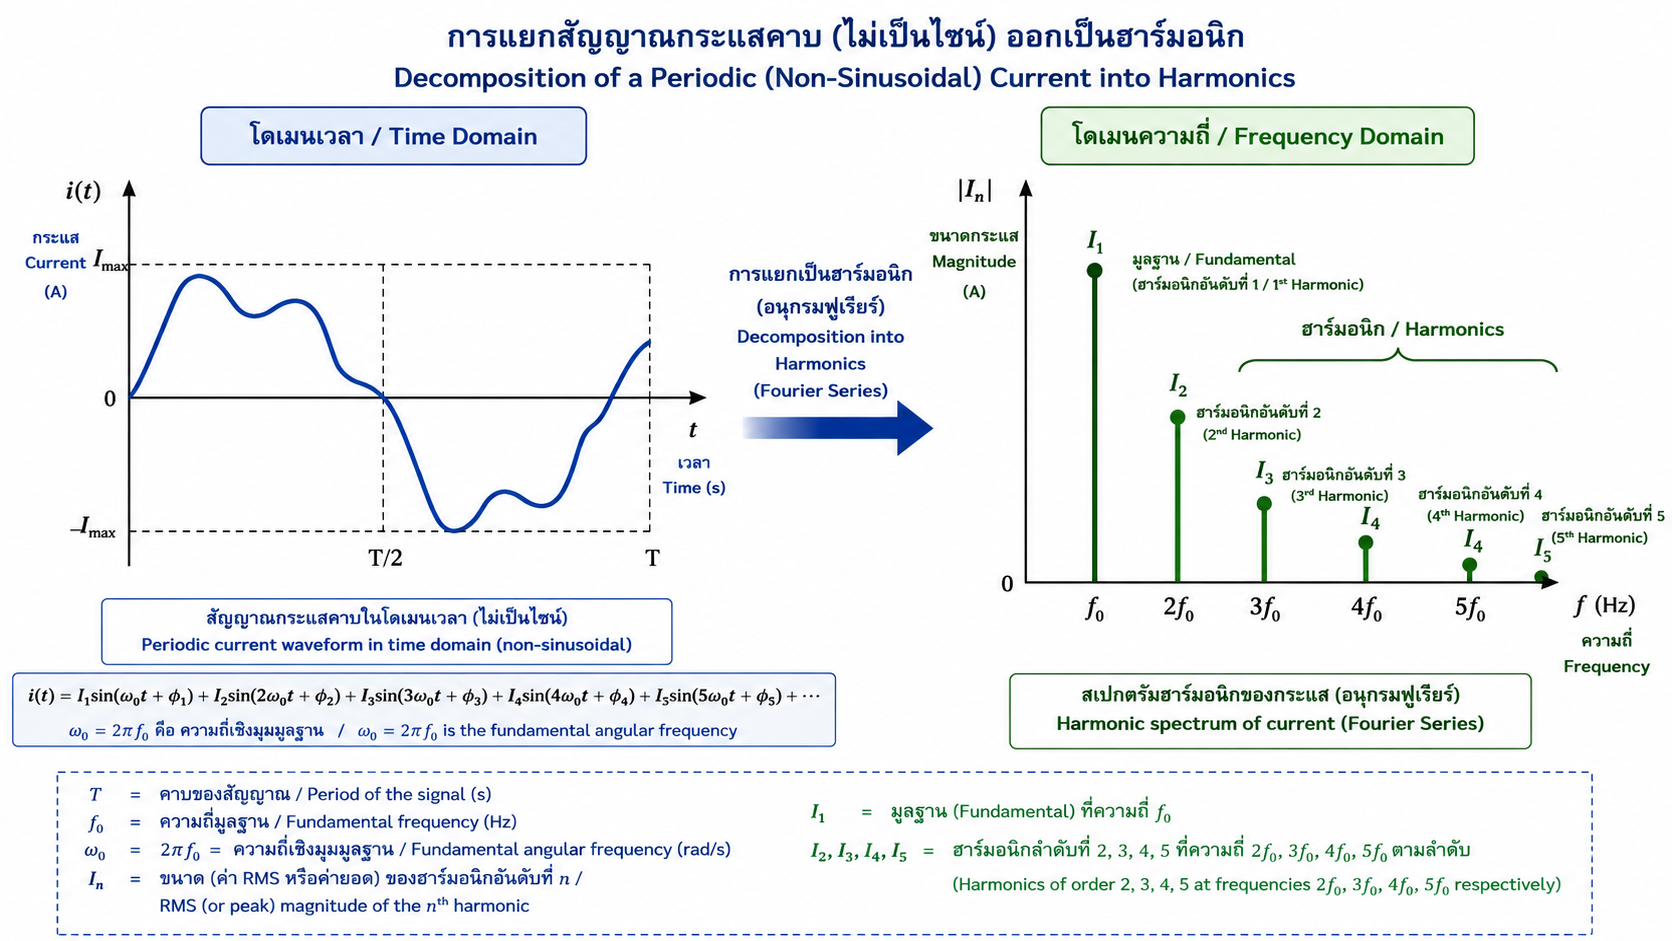
\includegraphics[width=0.8\textwidth]{images/chapter5/figure-01.png}
    \caption{ความเชื่อมโยงระหว่างรูปคลื่นในโดเมนเวลาและสเปกตรัมความถี่}
\end{figure}



\subsection{7.2 รูปคลื่นไซน์ รูปคลื่นสี่เหลี่ยม รูปคลื่นสามเหลี่ยม และรูปคลื่นฟันเลื่อย}

รูปคลื่นมาตรฐานทั้งสี่ชนิดมีประโยชน์อย่างมากในการเรียนรู้ เพราะแสดงให้เห็นโดยตรงว่า “ความคม” และ “ความไม่ต่อเนื่อง” ของรูปคลื่นสัมพันธ์กับการลดลงของแอมพลิจูดฮาร์มอนิกอย่างไร

\subsubsection{7.2.1 รูปคลื่นไซน์}

รูปคลื่นไซน์บริสุทธิ์เขียนได้เป็น

\[
x(t)=X_m\sin(\omega_0 t+\phi)
\]

โดย $X_m$ คือค่าสูงสุดหรือ peak value และ $\phi$ คือมุมเฟส หากเป็นไซน์บริสุทธิ์ที่ไม่มี DC สเปกตรัมจะมีเพียงองค์ประกอบที่ความถี่มูลฐานเท่านั้น

ค่าประสิทธิผลของไซน์คือ

\[
X_{\mathrm{rms}}=\frac{X_m}{\sqrt{2}}
\]

\subsubsection{7.2.2 รูปคลื่นสี่เหลี่ยมสมมาตร}

พิจารณารูปคลื่นสี่เหลี่ยมสมมาตรที่มีค่า $+X_m$ และ $-X_m$ อย่างละครึ่งคาบ และมีค่าเฉลี่ยเป็นศูนย์ เนื่องจากเป็นฟังก์ชันคี่ จึงเหลือเฉพาะพจน์ไซน์

\[
x(t)=\frac{4X_m}{\pi}\left(\sin\omega_0 t+\frac{1}{3}\sin3\omega_0 t+\frac{1}{5}\sin5\omega_0 t+\cdots\right)
\]

\textbf{คุณลักษณะสำคัญ}

\begin{itemize}
    \item มีเฉพาะฮาร์มอนิกลำดับคี่ $1,3,5,\ldots$
    \item แอมพลิจูด peak ของฮาร์มอนิกลำดับ $n$ ลดลงประมาณ $1/n$
    \item การลดลงแบบ $1/n$ ค่อนข้างช้า จึงมีฮาร์มอนิกลำดับสูงที่มีนัยสำคัญ
    \item เนื่องจากมีจุดไม่ต่อเนื่อง การประมาณด้วยจำนวนพจน์จำกัดจะเกิด Gibbs phenomenon ใกล้จุดกระโดด
\end{itemize}

\subsubsection{7.2.3 รูปคลื่นสามเหลี่ยมสมมาตร}

รูปคลื่นสามเหลี่ยมสมมาตรที่มีค่า peak $\pm X_m$ สามารถเขียนในรูปอนุกรมไซน์แบบหนึ่งได้เป็น

\[
x(t)=\frac{8X_m}{\pi^2}\left(\sin\omega_0 t-\frac{1}{3^2}\sin3\omega_0 t+\frac{1}{5^2}\sin5\omega_0 t-\cdots\right)
\]

\textbf{คุณลักษณะสำคัญ}

\begin{itemize}
    \item มีเฉพาะฮาร์มอนิกลำดับคี่
    \item แอมพลิจูดลดลงประมาณ $1/n^2$
    \item ลดลงเร็วกว่ารูปคลื่นสี่เหลี่ยม จึงมีความเพี้ยนน้อยกว่าเมื่อเทียบที่สเกลเดียวกัน
    \item รูปคลื่นต่อเนื่อง แต่ความชันเปลี่ยนอย่างฉับพลันที่ยอดและจุดต่ำสุด
\end{itemize}

\subsubsection{7.2.4 รูปคลื่นฟันเลื่อยสมมาตรรอบศูนย์}

สำหรับ sawtooth แบบสมมาตรรอบศูนย์ที่เพิ่มเชิงเส้นจาก $-X_m$ ไป $+X_m$ ภายในหนึ่งคาบ อนุกรมฟูเรียร์รูปหนึ่งคือ

\[
x(t)=\frac{2X_m}{\pi}\left(\sin\omega_0 t-\frac{1}{2}\sin2\omega_0 t+\frac{1}{3}\sin3\omega_0 t-\cdots\right)
\]

เครื่องหมายอาจเปลี่ยนตามการเลือกจุดกำเนิดเวลาและทิศทางของ sawtooth แต่สาระสำคัญคือ

\begin{itemize}
    \item มีทั้งฮาร์มอนิกลำดับคู่และคี่
    \item แอมพลิจูดลดลงประมาณ $1/n$
    \item มีจุดกระโดดหนึ่งครั้งต่อคาบ จึงมีพลังงานกระจายไปยังฮาร์มอนิกลำดับสูงมากกว่ารูปคลื่นสามเหลี่ยม
\end{itemize}

\subsubsection{7.2.5 ตารางเปรียบเทียบรูปคลื่นมาตรฐาน}

\begin{table}[htbp]
    \centering
    \small
    \begin{tabularx}{\textwidth}{>{\raggedright\arraybackslash}p{0.16\textwidth} >{\raggedright\arraybackslash}p{0.16\textwidth} >{\raggedright\arraybackslash}X >{\centering\arraybackslash}p{0.16\textwidth} >{\raggedright\arraybackslash}p{0.20\textwidth}}
        \hline
        \textbf{รูปคลื่น} & \textbf{ฮาร์มอนิกเด่น} & \textbf{การลดลงของแอมพลิจูด} & \textbf{$X_{\mathrm{rms}}$ เมื่อ peak = $X_m$} & \textbf{THD เชิงทฤษฎีของรูปคลื่นอุดมคติ*} \\
        \hline
        ไซน์ & มูลฐานเท่านั้น & ไม่มีฮาร์มอนิก & $X_m/\sqrt{2}$ & 0\% \\
        สี่เหลี่ยมสมมาตร & คี่ & $1/n$ & $X_m$ & ประมาณ 48.34\% \\
        สามเหลี่ยมสมมาตร & คี่ & $1/n^2$ & $X_m/\sqrt{3}$ & ประมาณ 12.12\% \\
        ฟันเลื่อยสมมาตร & คู่และคี่ & $1/n$ & $X_m/\sqrt{3}$ & ประมาณ 80.31\% \\
        \hline
    \end{tabularx}
\end{table}

* ค่า THD ในตารางคำนวณจากองค์ประกอบฮาร์มอนิกทั้งหมดของรูปคลื่นอุดมคติ โดยไม่นับ DC และอ้างองค์ประกอบมูลฐานเป็นตัวหาร ไม่ใช่ “เกณฑ์มาตรฐาน” ของระบบไฟฟ้า

% [รูปที่ 2: เปรียบเทียบรูปคลื่นมาตรฐานและการลดลงของฮาร์มอนิก]
% ประเภทภาพ: Graph / Infographic
% ตำแหน่งที่แนะนำ: หลังตารางเปรียบเทียบรูปคลื่นมาตรฐาน
% วัตถุประสงค์การเรียนรู้: แสดงความสัมพันธ์ระหว่างความเรียบของรูปคลื่นกับอัตราการลดลงของฮาร์มอนิก
% คำอธิบายภาพ: แบ่งเป็นสี่แถว แต่ละแถวมีกราฟเวลาและสเปกตรัมของ sine, square, triangle, sawtooth ที่สเกลเดียวกัน
% องค์ประกอบที่ต้องมี: waveform, spectrum, harmonic order, เส้นแนวโน้ม 1/n และ 1/n²
% ข้อความหรือป้ายกำกับ: “Sine”, “Square”, “Triangle”, “Sawtooth”, “odd harmonics”, “all harmonics”, “1/n”, “1/n²”
% ภาษาของป้ายกำกับ: ไทยและอังกฤษ
% สัดส่วนภาพ: 16:9
% Image Generation Prompt: Four-row engineering infographic comparing sine, symmetric square, symmetric triangle, and symmetric sawtooth waveforms. For each row show the time-domain waveform and a discrete harmonic magnitude spectrum. Highlight that square wave has odd harmonics decaying as 1/n, triangle has odd harmonics decaying as 1/n^2, sawtooth has even and odd harmonics decaying as 1/n, and sine has only the fundamental. White background, clean textbook vector graphics, bilingual Thai-English labels, 16:9.
% Graph Generation Prompt: Generate normalized waveforms with peak ±1 over two periods and corresponding normalized Fourier coefficient magnitude spectra up to harmonic order 15. Use consistent axes. Label harmonic order n and normalized magnitude.
% Alt Text: สี่ชุดกราฟเปรียบเทียบ sine, square, triangle และ sawtooth พร้อมสเปกตรัม แสดงว่ารูปสามเหลี่ยมมีฮาร์มอนิกลดลงเร็วที่สุดในกลุ่มรูปคลื่นไม่เป็นไซน์

\begin{figure}[htbp]
    \centering
    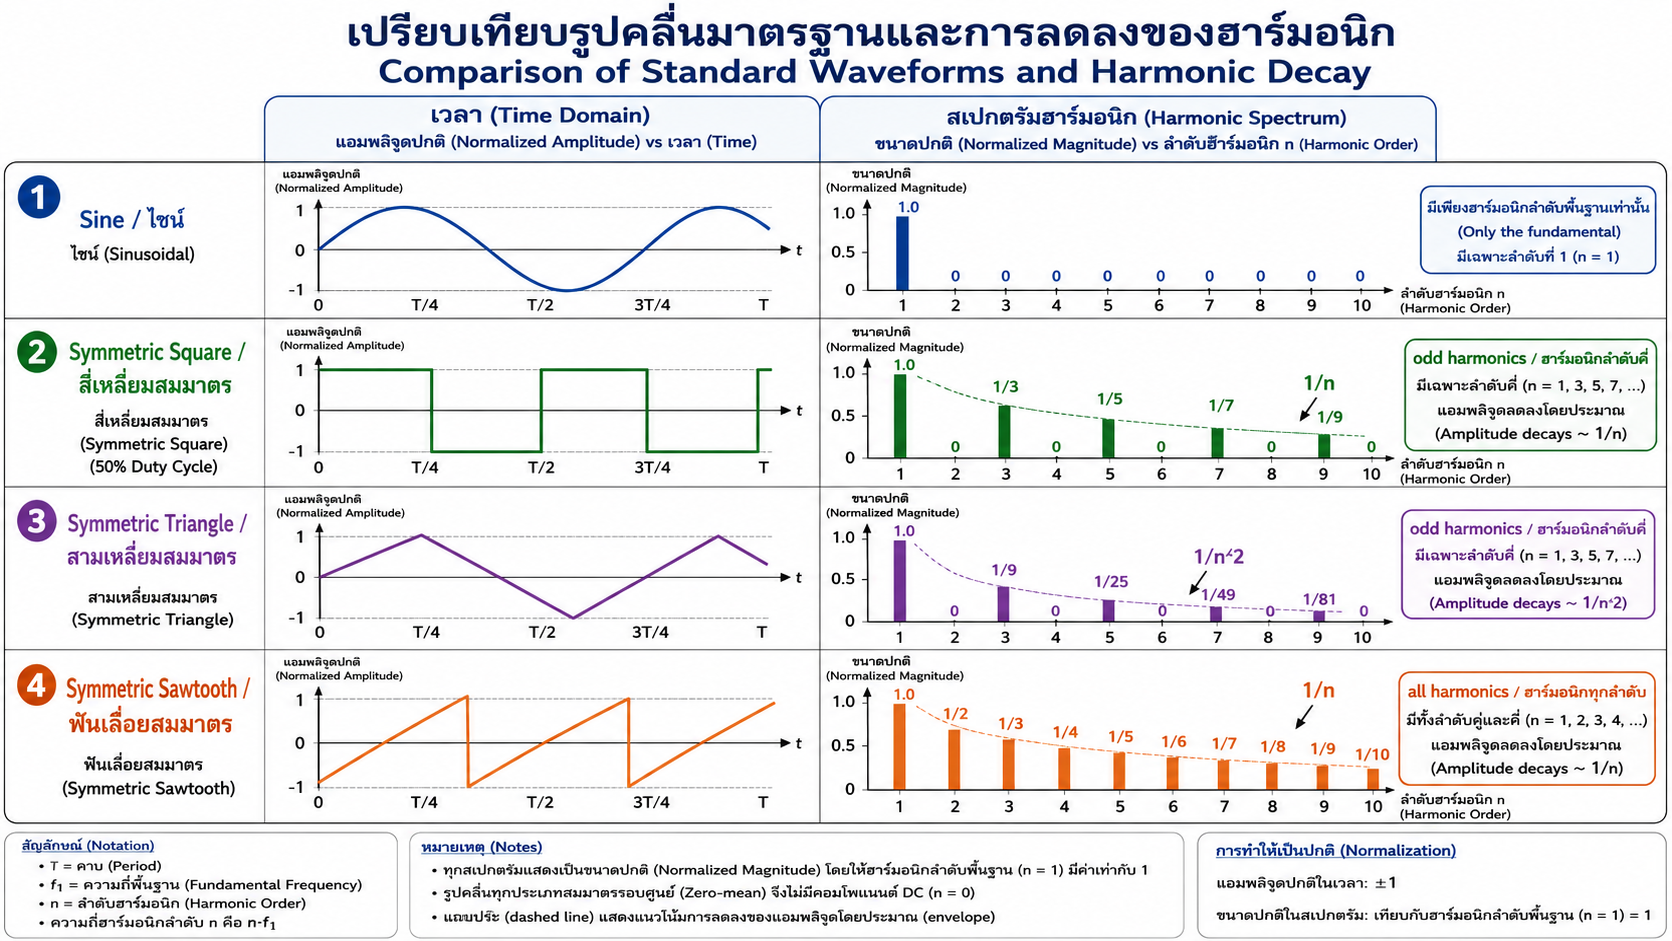
\includegraphics[width=0.8\textwidth]{images/chapter5/figure-02.png}
    \caption{เปรียบเทียบรูปคลื่นมาตรฐานและการลดลงของฮาร์มอนิก}
\end{figure}



\subsection{7.3 การวิเคราะห์ฮาร์มอนิกของรูปคลื่นไฟฟ้า}

\subsubsection{7.3.1 รูปทั่วไปของอนุกรมฟูเรียร์}

สำหรับสัญญาณเป็นคาบ $x(t)$ คาบ $T$ รูปตรีโกณมิติทั่วไปคือ

\[
x(t)=\frac{a_0}{2}+\sum_{n=1}^{\infty}\left[a_n\cos(n\omega_0 t)+b_n\sin(n\omega_0 t)\right]
\]

โดย

\[
a_0=\frac{2}{T}\int_{t_0}^{t_0+T}x(t)\,dt
\]

\[
a_n=\frac{2}{T}\int_{t_0}^{t_0+T}x(t)\cos(n\omega_0 t)\,dt
\]

\[
b_n=\frac{2}{T}\int_{t_0}^{t_0+T}x(t)\sin(n\omega_0 t)\,dt
\]

\textbf{ที่มา:} สมการเกิดจากสมบัติออร์โทโกนัลของไซน์และโคไซน์บนช่วงหนึ่งคาบ ทำให้สามารถแยกค่าสัมประสิทธิ์ของแต่ละความถี่ออกจากกันได้

\textbf{ความหมายของตัวแปร}

\begin{itemize}
    \item $a_0/2$ คือ DC component หรือค่าเฉลี่ย
    \item $a_n$ คือสัมประสิทธิ์โคไซน์ของฮาร์มอนิกลำดับที่ $n$
    \item $b_n$ คือสัมประสิทธิ์ไซน์ของฮาร์มอนิกลำดับที่ $n$
    \item $n\omega_0$ คือความถี่เชิงมุมของฮาร์มอนิกลำดับที่ $n$
\end{itemize}

\textbf{เงื่อนไขการใช้:} เหมาะกับสัญญาณเป็นคาบที่มีคุณสมบัติทางคณิตศาสตร์เพียงพอสำหรับการขยายเป็นอนุกรมฟูเรียร์ เช่น มีจำนวนจุดไม่ต่อเนื่องจำกัดในหนึ่งคาบและอินทิเกรตได้เป็นช่วง ๆ

\subsubsection{7.3.2 รูปแอมพลิจูด–เฟส}

พจน์ของฮาร์มอนิกลำดับที่ $n$ สามารถเขียนเป็น

\[
\begin{aligned}
    a_n\cos(n\omega_0 t)+b_n\sin(n\omega_0 t) \\
    =A_n\cos(n\omega_0 t-\theta_n)
\end{aligned}
\]

เมื่อ

\[
A_n=\sqrt{a_n^2+b_n^2}
\]

และ

\[
\theta_n=\operatorname{atan2}(b_n,a_n)
\]

การใช้ $\operatorname{atan2}$ ช่วยระบุควอดแรนต์ของมุมได้ถูกต้องกว่าการใช้ $\tan^{-1}(b_n/a_n)$ เพียงอย่างเดียว

\textbf{ความหมายทางกายภาพ:} $A_n$ บอก “ขนาด” ขององค์ประกอบความถี่ ส่วน $\theta_n$ บอกตำแหน่งเฟสขององค์ประกอบนั้นเมื่อเทียบกับแกนอ้างอิงเวลา

\subsubsection{7.3.3 สเปกตรัมขนาดแบบ peak และ RMS}

ในวิชาคณิตศาสตร์ ฟูเรียร์มักใช้ $A_n$ เป็น peak amplitude แต่ในวิศวกรรมกำลังมักรายงานขนาดฮาร์มอนิกเป็น RMS ดังนั้นต้องระบุชนิดของขนาดให้ชัดเจน

สำหรับองค์ประกอบไซน์หรือโคไซน์หนึ่งความถี่

\[
X_{n,\mathrm{rms}}=\frac{A_n}{\sqrt{2}}
\]

จึงควรหลีกเลี่ยงการนำ peak amplitude ไปใช้ในสูตร THD ที่กำหนดด้วย RMS โดยไม่แปลงหน่วยก่อน ถึงแม้อัตราส่วนบางกรณีจะให้ค่าเท่ากันหากทุกพจน์ใช้ชนิดเดียวกัน แต่การกำหนดมาตรฐานการคำนวณให้ชัดเจนช่วยลดความผิดพลาด

\subsubsection{7.3.4 Harmonic order กับความถี่จริง}

ถ้าระบบมี $f_0=50$ Hz

\begin{table}[htbp]
    \centering
    \begin{tabular}{r r}
        \hline
        \textbf{Harmonic order} & \textbf{ความถี่} \\
        \hline
        1 & 50 Hz \\
        2 & 100 Hz \\
        3 & 150 Hz \\
        5 & 250 Hz \\
        7 & 350 Hz \\
        11 & 550 Hz \\
        13 & 650 Hz \\
        \hline
    \end{tabular}
\end{table}

ในระบบ 60 Hz ให้คูณลำดับฮาร์มอนิกด้วย 60 แทน การระบุ “ลำดับฮาร์มอนิก” จึงสะดวกต่อการเปรียบเทียบระบบที่มีความถี่มูลฐานต่างกัน

\subsubsection{ตัวอย่างที่ 1: อ่านองค์ประกอบฮาร์มอนิกจากสมการรูปคลื่น}

\textbf{ตัวอย่างเพิ่มเติมเพื่อการเรียนรู้}

กำหนดกระแส

\[
i(t)=10\sqrt{2}\sin(2\pi 50t)+3\sqrt{2}\sin(2\pi 150t-20^\circ)+1.5\sqrt{2}\sin(2\pi 250t+30^\circ)\ \text{A}
\]

จงระบุความถี่มูลฐาน ลำดับฮาร์มอนิก ขนาด RMS และเฟสของแต่ละองค์ประกอบ

\textbf{ขั้นที่ 1 วิเคราะห์โจทย์} \\
รูปคลื่นประกอบด้วยไซน์สามความถี่ 50, 150 และ 250 Hz

\textbf{ขั้นที่ 2 กำหนดความถี่มูลฐาน}

\[
f_0=50\ \text{Hz}
\]

\textbf{ขั้นที่ 3 หา harmonic order}

\[
150/50=3,\qquad 250/50=5
\]

ดังนั้นมี fundamental, 3rd และ 5th harmonic

\textbf{ขั้นที่ 4 แปลง peak เป็น RMS} \\
เนื่องจาก coefficient ของไซน์เขียนเป็น $\sqrt{2}I_{\mathrm{rms}}$

\begin{itemize}
    \item $I_1=10$ A RMS, phase $0^\circ$
    \item $I_3=3$ A RMS, phase $-20^\circ$
    \item $I_5=1.5$ A RMS, phase $+30^\circ$
\end{itemize}

\textbf{ขั้นที่ 5 ตรวจสอบความสมเหตุสมผล} \\
ฮาร์มอนิกมีขนาดเล็กกว่ามูลฐาน จึงสอดคล้องกับรูปคลื่นที่ยังมีลักษณะพื้นฐาน 50 Hz แต่เกิดการเพี้ยน

\textbf{คำตอบ}

\begin{table}[htbp]
    \centering
    \begin{tabular}{l r r r}
        \hline
        \textbf{องค์ประกอบ} & \textbf{ความถี่} & \textbf{RMS} & \textbf{เฟส} \\
        \hline
        Fundamental & 50 Hz & 10 A & $0^\circ$ \\
        3rd harmonic & 150 Hz & 3 A & $-20^\circ$ \\
        5th harmonic & 250 Hz & 1.5 A & $+30^\circ$ \\
        \hline
    \end{tabular}
\end{table}

% [รูปที่ 3: การสังเคราะห์รูปคลื่นจาก fundamental, 3rd และ 5th harmonic]
% ประเภทภาพ: Graph
% ตำแหน่งที่แนะนำ: หลังตัวอย่างที่ 1
% วัตถุประสงค์การเรียนรู้: แสดงว่าการบวกฮาร์มอนิกเปลี่ยนรูปร่างของสัญญาณอย่างไร
% คำอธิบายภาพ: กราฟบนแสดงองค์ประกอบ 50, 150, 250 Hz แยกเส้น กราฟล่างแสดงผลรวม
% องค์ประกอบที่ต้องมี: แกนเวลา ms, กระแส A, legend ของ fundamental/3rd/5th/sum
% ข้อความหรือป้ายกำกับ: “Fundamental 50 Hz”, “3rd 150 Hz”, “5th 250 Hz”, “Resultant waveform”
% ภาษาของป้ายกำกับ: ไทยและอังกฤษ
% สัดส่วนภาพ: 16:9
% Image Generation Prompt: Engineering mathematics graph showing three sinusoidal current components at 50 Hz, 150 Hz, and 250 Hz and their summed distorted waveform. Use two panels: individual harmonics on top and resultant waveform below. Precise axes in milliseconds and amperes, bilingual Thai-English labels, white background, textbook vector style, 16:9.
% Graph Generation Prompt: Plot i1(t)=10√2 sin(2π50t), i3(t)=3√2 sin(2π150t−20°), i5(t)=1.5√2 sin(2π250t+30°), and i(t)=i1+i3+i5 from 0 to 40 ms. Use amperes and milliseconds.
% Alt Text: กราฟแสดงไซน์สามความถี่และผลรวมที่เกิดเป็นกระแสผิดรูปจากฮาร์มอนิกอันดับ 3 และ 5

\begin{figure}[htbp]
    \centering
    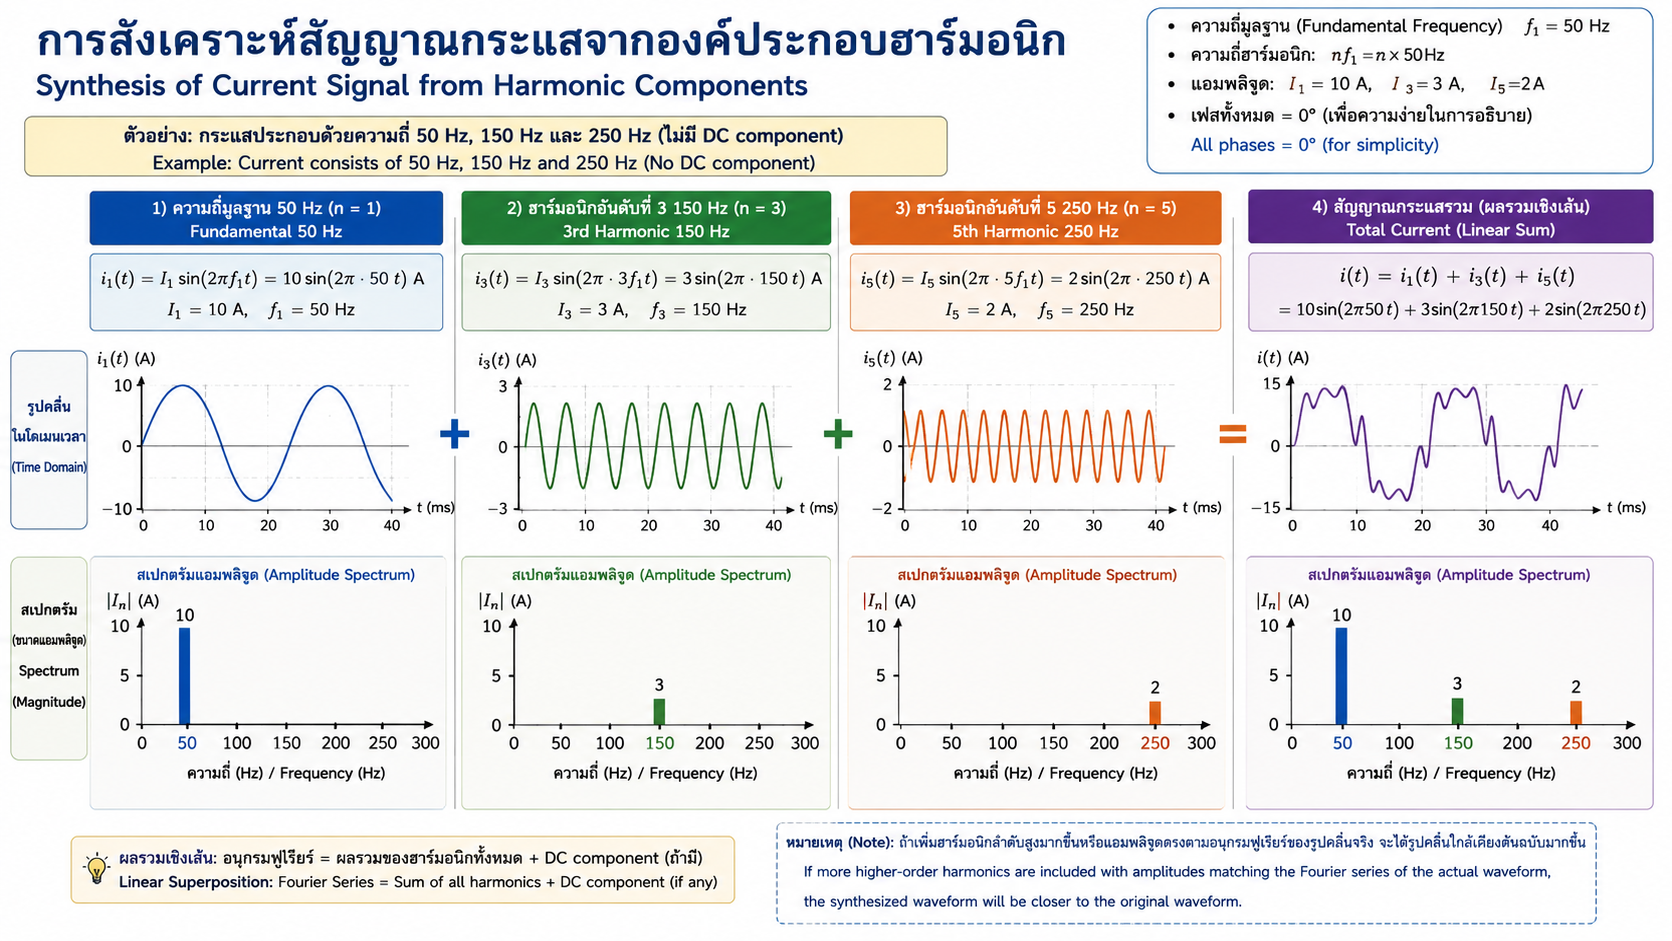
\includegraphics[width=0.8\textwidth]{images/chapter5/figure-03.png}
    \caption{การสังเคราะห์รูปคลื่นจาก fundamental, 3rd และ 5th harmonic}
\end{figure}



\subsection{7.4 ความสัมพันธ์ระหว่างอนุกรมฟูเรียร์กับคุณภาพกำลังไฟฟ้า}

\subsubsection{7.4.1 จากโหลดไม่เชิงเส้นสู่แรงดันเพี้ยน}

พิจารณาระบบจ่ายไฟอย่างง่ายที่มีแรงดันต้นทางเชิงอุดมคติ $v_s(t)$ และอิมพีแดนซ์ระบบ $Z_s$ หากโหลดไม่เชิงเส้นดึงกระแส

\[
i(t)=\sum_{n=1}^{\infty} i_n(t)
\]

กระแสแต่ละฮาร์มอนิกจะสร้างแรงดันตกคร่อมที่ความถี่เดียวกันผ่านอิมพีแดนซ์ของระบบ ดังนั้นแรงดันที่จุดโหลดสามารถมองเชิงแนวคิดได้ว่า

\[
V_n \approx I_n Z_s(n\omega_0)
\]

สมการนี้ไม่ใช่แบบจำลองระบบกำลังเต็มรูปแบบ แต่ช่วยอธิบายหลักสำคัญว่า \textbf{ฮาร์มอนิกกระแสทำให้เกิดฮาร์มอนิกแรงดันได้เมื่อระบบมีอิมพีแดนซ์ไม่เป็นศูนย์}

\subsubsection{7.4.2 PCC และมุมมองของมาตรฐาน}

IEEE 519-2022 กำหนดเป้าหมายสำหรับการออกแบบระบบที่มีทั้งโหลดเชิงเส้นและไม่เชิงเส้น และประเมินขีดจำกัดความเพี้ยนของแรงดันและกระแสแบบ steady-state ที่ \textbf{Point of Common Coupling (PCC)} แนวคิดนี้มีความสำคัญต่อผู้เรียน เพราะทำให้ไม่สับสนระหว่าง

\begin{enumerate}
    \item รูปคลื่นภายในอุปกรณ์หนึ่งชิ้น
    \item กระแสที่อุปกรณ์ฉีดเข้าสู่ระบบ
    \item ผลรวมของโหลดหลายชนิดที่ PCC
    \item ความเพี้ยนของแรงดันระบบที่ผู้ใช้อื่นร่วมกันได้รับ
\end{enumerate}

ดังนั้นค่า THD ที่วัดจากอุปกรณ์เดี่ยวในห้องทดลองไม่ควรถูกนำไปสรุปว่า “ผ่านหรือไม่ผ่าน IEEE 519” โดยตรง หากยังไม่ได้กำหนดตำแหน่งวัด เงื่อนไขระบบ และตัวชี้วัดที่มาตรฐานกำหนด

\subsubsection{7.4.3 ฮาร์มอนิกกับ power quality ไม่ใช่เรื่องเดียวกันทั้งหมด}

คุณภาพกำลังไฟฟ้ายังครอบคลุมความถี่ แรงดันตก/เกินชั่วขณะ flicker interruption unbalance transient และปรากฏการณ์อื่น การวิเคราะห์ฮาร์มอนิกจึงเป็นเพียงส่วนหนึ่งของ power quality แต่เป็นส่วนที่เหมาะกับการใช้ Fourier analysis อย่างเด่นชัด

% [รูปที่ 4: เส้นทางการเกิดฮาร์มอนิกในระบบไฟฟ้า]
% ประเภทภาพ: Block Diagram / Technical Illustration
% ตำแหน่งที่แนะนำ: หัวข้อ 7.4
% วัตถุประสงค์การเรียนรู้: แสดงเหตุ–ผลจากโหลดไม่เชิงเส้นไปยังความเพี้ยนที่ PCC
% คำอธิบายภาพ: แหล่งจ่ายไซน์ → อิมพีแดนซ์ระบบ → PCC → โหลดไม่เชิงเส้น โดยมีลูกศร current harmonics ไหลจากโหลด และ voltage distortion เกิดที่ PCC
% องค์ประกอบที่ต้องมี: AC source, source impedance, PCC, nonlinear load, harmonic current arrows, distorted PCC voltage
% ข้อความหรือป้ายกำกับ: “Source”, “System impedance”, “PCC”, “Nonlinear load”, “Harmonic current”, “Voltage distortion”
% ภาษาของป้ายกำกับ: ไทยและอังกฤษ
% สัดส่วนภาพ: 16:9
% Image Generation Prompt: Clean electrical engineering block diagram illustrating harmonic propagation in a power system. Show an ideal sinusoidal AC source, source/system impedance, a labeled Point of Common Coupling (PCC), and a nonlinear load such as a rectifier or switching power supply. Show distorted harmonic current flowing from the load through the system impedance and resulting voltage distortion at the PCC. Bilingual Thai-English labels, white background, vector textbook style, 16:9.
% Alt Text: แผนภาพแสดงโหลดไม่เชิงเส้นสร้างกระแสฮาร์มอนิกซึ่งไหลผ่านอิมพีแดนซ์ระบบและทำให้แรงดันที่ PCC เพี้ยน

\begin{figure}[htbp]
    \centering
    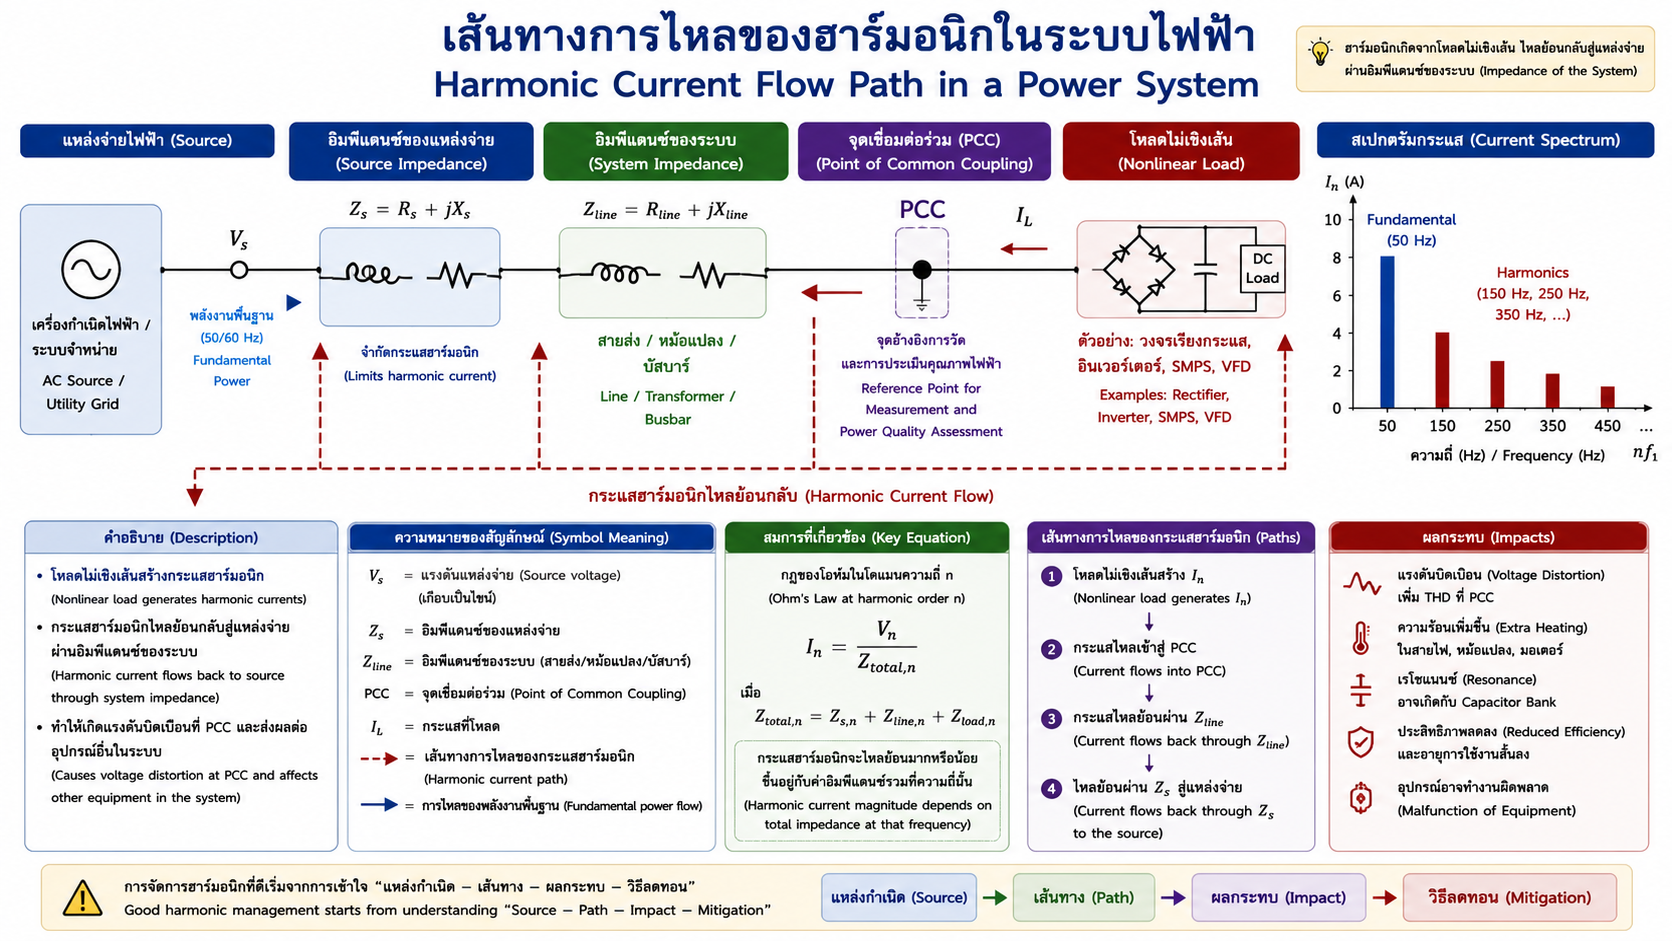
\includegraphics[width=0.8\textwidth]{images/chapter5/figure-04.png}
    \caption{เส้นทางการเกิดฮาร์มอนิกในระบบไฟฟ้า}
\end{figure}


\subsection{7.5 ค่าประสิทธิผลของสัญญาณไฟฟ้า}

\subsubsection{7.5.1 ความหมายของ RMS}

ค่าประสิทธิผล หรือ \textbf{Root Mean Square (RMS)} ของสัญญาณเป็นคาบ $x(t)$ นิยามโดย

\[
X_{\mathrm{rms}}=\sqrt{\frac{1}{T}\int_{t_0}^{t_0+T}x^2(t)\,dt}
\]

สมการนี้มีขั้นตอนตามชื่อโดยตรง

\begin{enumerate}
    \item \textbf{Square:} ยกกำลังสองสัญญาณ เพื่อทำให้ค่าบวกและลบไม่หักล้างกัน
    \item \textbf{Mean:} หาเฉลี่ยตลอดหนึ่งคาบ
    \item \textbf{Root:} ถอดรากที่สองเพื่อให้หน่วยกลับมาเหมือนปริมาณเดิม
\end{enumerate}

หาก $x(t)$ เป็นแรงดัน หน่วยของ $X_{\mathrm{rms}}$ คือโวลต์ หากเป็นกระแส หน่วยคือแอมแปร์

\subsubsection{7.5.2 ความหมายทางกายภาพ}

สำหรับแรงดันหรือกระแสที่จ่ายให้ตัวต้านทาน RMS คือค่ากระแสตรงที่ก่อให้เกิดกำลังเฉลี่ยหรือผลความร้อนเท่ากัน ตัวอย่างเช่น ถ้ากระแส AC มี $I_{\mathrm{rms}}=5$ A ไหลผ่านตัวต้านทาน $R$ กำลังเฉลี่ยที่ตัวต้านทานรับคือ

\[
P=I_{\mathrm{rms}}^2R
\]

แม้ว่ารูปคลื่นกระแสจะไม่เป็นไซน์ก็ตาม ตราบใดที่ $R$ เป็นตัวต้านทานเชิงอุดมคติและใช้ค่า true RMS ของกระแสนั้น

\subsubsection{7.5.3 RMS จากองค์ประกอบฟูเรียร์: Parseval relation}

ถ้าสัญญาณเขียนได้เป็น

\[
x(t)=X_{\mathrm{DC}}+\sum_{n=1}^{\infty}x_n(t)
\]

โดย $x_n(t)$ เป็นไซน์/โคไซน์ของฮาร์มอนิกลำดับที่ $n$ และองค์ประกอบแต่ละความถี่ตั้งฉากกันในความหมายของอินทิกรัลตลอดหนึ่งคาบ จะได้

\[
X_{\mathrm{rms}}^2=X_{\mathrm{DC}}^2+\sum_{n=1}^{\infty}X_{n,\mathrm{rms}}^2
\]

หรือ

\[
X_{\mathrm{rms}}=\sqrt{X_{\mathrm{DC}}^2+X_{1,\mathrm{rms}}^2+X_{2,\mathrm{rms}}^2+\cdots}
\]

\textbf{ความหมายสำคัญ:} RMS รวมไม่ได้เท่ากับผลบวกธรรมดาของ RMS แต่เป็น \textbf{รากที่สองของผลบวกกำลังสอง} ขององค์ประกอบที่ออร์โทโกนัลกัน

หากใช้สัมประสิทธิ์ตรีโกณมิติแบบ peak

\[
x(t)=\frac{a_0}{2}+\sum_{n=1}^{\infty}[a_n\cos(n\omega_0t)+b_n\sin(n\omega_0t)]
\]

จะได้

\[
X_{\mathrm{rms}}^2=\left(\frac{a_0}{2}\right)^2+\frac{1}{2}\sum_{n=1}^{\infty}(a_n^2+b_n^2)
\]

\textbf{สมมติฐานและข้อจำกัด:} สมการนี้ใช้กับสัญญาณเป็นคาบที่มี Fourier series และค่ากำลังเฉลี่ยจำกัด หากเป็นสัญญาณ transient หรือไม่เป็นคาบ ควรใช้กรอบ Fourier transform หรือวิธีวิเคราะห์สัญญาณอื่น

\subsubsection{ตัวอย่างที่ 2: คำนวณ RMS จากฮาร์มอนิก}

\textbf{ตัวอย่างเพิ่มเติมเพื่อการเรียนรู้}

กระแสหนึ่งมีองค์ประกอบ RMS ดังนี้

\begin{itemize}
    \item fundamental: $I_1=10$ A
    \item 3rd harmonic: $I_3=3$ A
    \item 5th harmonic: $I_5=1.5$ A
    \item 7th harmonic: $I_7=1$ A
\end{itemize}

ไม่มี DC component จงหา $I_{\mathrm{rms}}$

\textbf{ขั้นที่ 1 วิเคราะห์ระบบ} \\
ฮาร์มอนิกแต่ละลำดับเป็นความถี่ต่างกัน จึงรวมแบบ root-sum-square

\textbf{ขั้นที่ 2 เลือกสมการ}

\[
I_{\mathrm{rms}}=\sqrt{I_1^2+I_3^2+I_5^2+I_7^2}
\]

\textbf{ขั้นที่ 3 แทนค่า}

\[
I_{\mathrm{rms}}=\sqrt{10^2+3^2+1.5^2+1^2}
\]

\[
=\sqrt{100+9+2.25+1}
\]

\[
=\sqrt{112.25}=10.59\ \text{A}
\]

\textbf{ขั้นที่ 4 ตรวจสอบหน่วยและความสมเหตุสมผล} \\
ค่า RMS รวมต้องมากกว่า 10 A เพราะมีฮาร์มอนิกเพิ่มเข้ามา แต่ไม่ควรเป็น $10+3+1.5+1=15.5$ A เพราะองค์ประกอบไม่อยู่เฟสและความถี่เดียวกันตลอดเวลา

\textbf{คำตอบ:}

\[
\boxed{I_{\mathrm{rms}}\approx10.59\ \text{A}}
\]

\subsubsection{7.5.4 RMS ของรูปคลื่นมาตรฐาน}

\begin{itemize}
    \item ไซน์ peak $X_m$:
\end{itemize}

\[
X_{\mathrm{rms}}=\frac{X_m}{\sqrt{2}}
\]

\begin{itemize}
    \item สี่เหลี่ยมสมมาตร $\pm X_m$:
\end{itemize}

\[
X_{\mathrm{rms}}=X_m
\]

\begin{itemize}
    \item สามเหลี่ยมสมมาตร $\pm X_m$:
\end{itemize}

\[
X_{\mathrm{rms}}=\frac{X_m}{\sqrt{3}}
\]

\begin{itemize}
    \item sawtooth สมมาตร $\pm X_m$:
\end{itemize}

\[
X_{\mathrm{rms}}=\frac{X_m}{\sqrt{3}}
\]

\subsubsection{7.5.5 ค่าเฉลี่ยไม่ใช่ RMS}

รูปคลื่นสี่เหลี่ยมสมมาตร $+10$ V และ $-10$ V มีค่าเฉลี่ยเท่ากับศูนย์ แต่ RMS เท่ากับ 10 V ดังนั้นการใช้ค่าเฉลี่ยเพื่อประเมินผลความร้อนของ AC จะผิดพลาดอย่างมาก



\subsection{7.6 กำลังไฟฟ้าเฉลี่ยและกำลังไฟฟ้าในรูปคลื่นไม่เป็นไซน์}

\subsubsection{7.6.1 นิยามกำลังทันทีและกำลังเฉลี่ย}

กำลังไฟฟ้าทันทีคือ

\[
p(t)=v(t)i(t)
\]

กำลังไฟฟ้าเฉลี่ยในหนึ่งคาบคือ

\[
P=\frac{1}{T}\int_{t_0}^{t_0+T}v(t)i(t)\,dt
\]

สมการนี้เป็นนิยามพื้นฐานที่ใช้ได้ทั้งกรณีไซน์และไม่เป็นไซน์

\subsubsection{7.6.2 กำลังเฉลี่ยเมื่อแรงดันและกระแสมีฮาร์มอนิก}

ให้

\[
v(t)=V_{\mathrm{DC}}+\sum_{n=1}^{\infty}v_n(t)
\]

และ

\[
i(t)=I_{\mathrm{DC}}+\sum_{n=1}^{\infty}i_n(t)
\]

ด้วยสมบัติออร์โทโกนัล องค์ประกอบต่างความถี่มีค่าเฉลี่ยของผลคูณเป็นศูนย์เมื่ออินทิเกรตตลอดคาบร่วม ดังนั้นกำลังเฉลี่ยสามารถเขียนได้เป็น

\[
P=V_{\mathrm{DC}}I_{\mathrm{DC}}+\sum_{n=1}^{\infty}V_{n,\mathrm{rms}}I_{n,\mathrm{rms}}\cos\phi_n
\]

เมื่อ $\phi_n$ คือมุมเฟสต่างระหว่างแรงดันและกระแสของฮาร์มอนิกลำดับเดียวกัน

\textbf{ความหมายทางกายภาพ:} 50 Hz ของแรงดันสร้างกำลังเฉลี่ยกับ 50 Hz ของกระแส, 150 Hz ของแรงดันสร้างกำลังเฉลี่ยกับ 150 Hz ของกระแส เป็นต้น ส่วนการคูณข้ามความถี่จะเฉลี่ยเป็นศูนย์ในช่วงคาบที่เหมาะสม

\subsubsection{7.6.3 Apparent power และ true power factor}

โดยทั่วไปกำหนด apparent power เป็น

\[
S=V_{\mathrm{rms}}I_{\mathrm{rms}}
\]

หน่วย volt-ampere (VA) และ true power factor เป็น

\[
\mathrm{PF}=\frac{P}{V_{\mathrm{rms}}I_{\mathrm{rms}}}
\]

สำหรับกรณีไซน์บริสุทธิ์ทั้งแรงดันและกระแส PF ลดรูปเป็น $\cos\phi$ แต่เมื่อรูปคลื่นไม่เป็นไซน์ การใช้เพียง $\cos\phi_1$ อาจไม่แทน true PF

\subsubsection{7.6.4 กรณีแรงดันเป็นไซน์ แต่กระแสเพี้ยน}

ถ้าแรงดันมีเฉพาะ fundamental และไม่มี DC

\[
v(t)=v_1(t)
\]

กำลังเฉลี่ยเกิดจาก fundamental current เท่านั้น

\[
P=V_1I_1\cos\phi_1
\]

แต่

\[
I_{\mathrm{rms}}=\sqrt{I_1^2+I_2^2+I_3^2+\cdots}
\]

ดังนั้น

\[
\mathrm{PF}=\frac{V_1I_1\cos\phi_1}{V_1I_{\mathrm{rms}}}
\]

\[
\mathrm{PF}=\frac{I_1}{I_{\mathrm{rms}}}\cos\phi_1
\]

เทอม

\[
\frac{I_1}{I_{\mathrm{rms}}}
\]

สะท้อนผลของ waveform distortion ขณะที่ $\cos\phi_1$ สะท้อน displacement ระหว่าง fundamental voltage และ fundamental current

\subsubsection{ตัวอย่างที่ 3: ตัวประกอบกำลังเมื่อกระแสมีฮาร์มอนิก}

\textbf{ตัวอย่างเพิ่มเติมเพื่อการเรียนรู้}

แรงดันจ่ายเป็นไซน์บริสุทธิ์ $V_1=230$ V RMS โหลดดึงกระแส

\begin{itemize}
    \item $I_1=8$ A RMS ที่ displacement factor $\cos\phi_1=0.90$
    \item $I_3=2.5$ A RMS
    \item $I_5=1.5$ A RMS
\end{itemize}

จงหากระแส RMS รวม กำลังจริง apparent power และ true PF

\textbf{ขั้นที่ 1 กระแส RMS รวม}

\[
I_{\mathrm{rms}}=\sqrt{8^2+2.5^2+1.5^2}
\]

\[
=\sqrt{64+6.25+2.25}=\sqrt{72.5}=8.51\ \text{A}
\]

\textbf{ขั้นที่ 2 กำลังจริง} \\
เพราะแรงดันมีเฉพาะ 50 Hz จึงมีเฉพาะ $V_1I_1\cos\phi_1$

\[
P=230(8)(0.90)=1656\ \text{W}
\]

\textbf{ขั้นที่ 3 apparent power}

\[
S=230(8.51)=1957.3\ \text{VA}
\]

\textbf{ขั้นที่ 4 true PF}

\[
\mathrm{PF}=\frac{1656}{1957.3}=0.846
\]

\textbf{การแปลความหมาย:} แม้ displacement factor ของ fundamental จะเป็น 0.90 แต่ true PF เหลือประมาณ 0.846 เนื่องจากฮาร์มอนิกเพิ่ม $I_{\mathrm{rms}}$ โดยไม่ได้สร้างกำลังจริงเพิ่มในกรณีที่แรงดันไม่มีฮาร์มอนิกสอดคล้องกัน

\textbf{คำตอบ}

\[
\boxed{I_{\mathrm{rms}}\approx8.51\ \text{A},\quad P=1.656\ \text{kW},\quad S\approx1.957\ \text{kVA},\quad PF\approx0.846}
\]

% [รูปที่ 5: กำลังไฟฟ้าในโดเมนฮาร์มอนิก]
% ประเภทภาพ: Infographic / Spectrum Diagram
% ตำแหน่งที่แนะนำ: หลังหัวข้อ 7.6.2
% วัตถุประสงค์การเรียนรู้: แสดงว่ากำลังเฉลี่ยจับคู่แรงดันและกระแสที่ฮาร์มอนิกลำดับเดียวกัน
% คำอธิบายภาพ: สเปกตรัมแรงดันด้านบนและกระแสด้านล่าง พร้อมลูกศรเชื่อม $V_1$ กับ $I_1$, $V_3$ กับ $I_3$, $V_5$ กับ $I_5$ และแสดงสูตร $P=\sum V_nI_n\cos\phi_n$
% องค์ประกอบที่ต้องมี: harmonic order, RMS magnitude, phase labels, matching arrows
% ข้อความหรือป้ายกำกับ: “Same-order harmonic power contribution”, “ต่างความถี่เฉลี่ยเป็นศูนย์”
% ภาษาของป้ายกำกับ: ไทยและอังกฤษ
% สัดส่วนภาพ: 16:9
% Image Generation Prompt: Engineering infographic illustrating average power in nonsinusoidal voltage and current. Show separate voltage and current harmonic spectra with matching arrows between V1-I1, V3-I3, V5-I5 and annotate P = sum(Vn_rms In_rms cos(phi_n)). Emphasize that cross-frequency products average to zero over a common period. White background, bilingual Thai-English labels, clean textbook vector style, 16:9.
% Alt Text: สเปกตรัมแรงดันและกระแสแสดงการจับคู่ฮาร์มอนิกลำดับเดียวกันในการคำนวณกำลังเฉลี่ย

\begin{figure}[htbp]
    \centering
    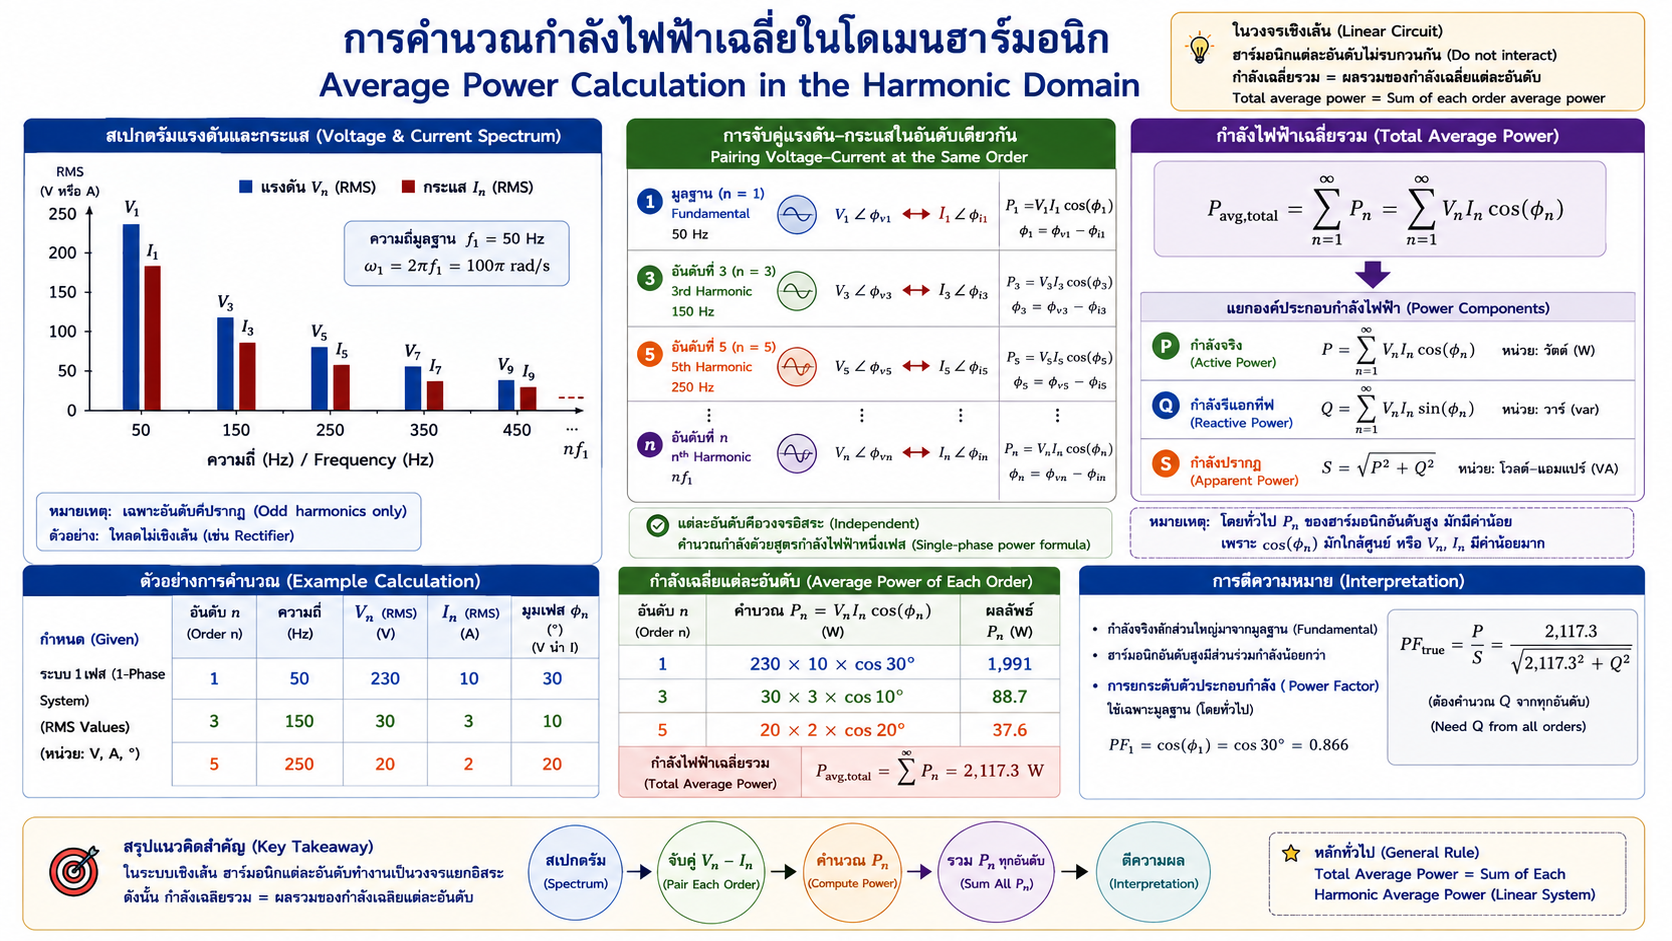
\includegraphics[width=0.8\textwidth]{images/chapter5/figure-05.png}
    \caption{กำลังไฟฟ้าในโดเมนฮาร์มอนิก}
\end{figure}



\subsection{7.7 การวิเคราะห์ Total Harmonic Distortion หรือ THD}

\subsubsection{7.7.1 นิยาม THD}

สำหรับแรงดันที่มี fundamental RMS เท่ากับ $V_1$ และฮาร์มอนิกตั้งแต่ลำดับที่ 2 ขึ้นไป

\[
\mathrm{THD}_V=\frac{\sqrt{V_2^2+V_3^2+V_4^2+\cdots}}{V_1}\times100\%
\]

สำหรับกระแส

\[
\mathrm{THD}_I=\frac{\sqrt{I_2^2+I_3^2+I_4^2+\cdots}}{I_1}\times100\%
\]

โดยทุก $V_n$ และ $I_n$ ต้องใช้ชนิดขนาดเดียวกัน โดยทั่วไปใช้ RMS

\subsubsection{7.7.2 ความสัมพันธ์ระหว่าง THD กับ RMS รวม}

หากไม่มี DC

\[
V_{\mathrm{rms}}^2=V_1^2+\sum_{n=2}^{\infty}V_n^2
\]

ดังนั้น

\[
V_{\mathrm{rms}}=V_1\sqrt{1+\mathrm{THD}_V^2}
\]

เมื่อ THD ในสมการนี้เขียนเป็นอัตราส่วน เช่น 0.05 ไม่ใช่ 5

ในทำนองเดียวกัน

\[
I_{\mathrm{rms}}=I_1\sqrt{1+\mathrm{THD}_I^2}
\]

\subsubsection{7.7.3 THD บอกอะไร และไม่บอกอะไร}

THD มีข้อดีคือสรุปความเพี้ยนเป็นตัวเลขเดียว แต่ไม่ได้บอกว่า

\begin{itemize}
    \item ฮาร์มอนิกลำดับใดเป็นตัวหลัก
    \item เฟสของฮาร์มอนิกเป็นอย่างไร
    \item มี interharmonic หรือไม่
    \item รูปคลื่นเกิด transient หรือไม่
    \item ตำแหน่งวัดอยู่ที่ใด
    \item ค่าเดียวกันเกิดจากสเปกตรัมที่แตกต่างกันมากเพียงใด
\end{itemize}

ดังนั้นในการวิเคราะห์ทางวิศวกรรมควรดู \textbf{ทั้งค่า THD และสเปกตรัมฮาร์มอนิก}

\subsubsection{7.7.4 THD กับ TDD ไม่ใช่สิ่งเดียวกัน}

ในการประเมินกระแสของระบบกำลังตามแนวทาง IEEE 519 มีการใช้ \textbf{Total Demand Distortion (TDD)} ซึ่งอ้างอิงกับ demand current ที่กำหนดตามมาตรฐาน ไม่ใช่ fundamental current ณ ขณะวัดเหมือน THD$_I$ การสอนระดับพื้นฐานจึงควรเน้นให้ผู้เรียนแยกคำสองคำนี้ออกจากกัน และไม่ใช้ THD$_I$ แทน TDD โดยอัตโนมัติ

\subsubsection{ตัวอย่างที่ 4: คำนวณ THD จากสเปกตรัมกระแส}

\textbf{ตัวอย่างเพิ่มเติมเพื่อการเรียนรู้}

จากตัวอย่างก่อนหน้า

\begin{itemize}
    \item $I_1=10$ A
    \item $I_3=3$ A
    \item $I_5=1.5$ A
    \item $I_7=1$ A
\end{itemize}

จงหา $\mathrm{THD}_I$

\textbf{ขั้นที่ 1 เลือกสมการ}

\[
\mathrm{THD}_I=\frac{\sqrt{I_3^2+I_5^2+I_7^2}}{I_1}\times100\%
\]

\textbf{ขั้นที่ 2 แทนค่า}

\[
\mathrm{THD}_I=\frac{\sqrt{3^2+1.5^2+1^2}}{10}\times100\%
\]

\[
=\frac{\sqrt{9+2.25+1}}{10}\times100\%
\]

\[
=\frac{3.5}{10}\times100\%=35\%
\]

\textbf{ขั้นที่ 3 ตรวจสอบด้วย RMS รวม}

\[
I_{\mathrm{rms}}=I_1\sqrt{1+0.35^2}
\]

\[
=10\sqrt{1.1225}=10.59\ \text{A}
\]

ตรงกับผลในตัวอย่างที่ 2

\textbf{คำตอบ:}

\[
\boxed{\mathrm{THD}_I=35\%}
\]

\subsubsection{7.7.5 THD ของรูปคลื่นสี่เหลี่ยมอุดมคติ}

รูปคลื่นสี่เหลี่ยมสมมาตร $\pm X_m$ มี RMS รวมเท่ากับ $X_m$ และ fundamental peak เท่ากับ $4X_m/\pi$ ดังนั้น fundamental RMS คือ

\[
X_1=\frac{4X_m}{\pi\sqrt{2}}
\]

จาก

\[
\mathrm{THD}=\frac{\sqrt{X_{\mathrm{rms}}^2-X_1^2}}{X_1}
\]

ได้

\[
\mathrm{THD}=\sqrt{\frac{\pi^2}{8}-1}
\]

\[
\mathrm{THD}\approx0.4834=48.34\%
\]

ค่าดังกล่าวช่วยให้เห็นว่ารูปคลื่นสี่เหลี่ยมที่ “ดูเป็นรูปทรงเรียบง่าย” ในโดเมนเวลา แท้จริงมีฮาร์มอนิกจำนวนมาก

% [รูปที่ 6: การคำนวณ THD จากสเปกตรัม]
% ประเภทภาพ: Infographic / Graph
% ตำแหน่งที่แนะนำ: หลังตัวอย่างที่ 4
% วัตถุประสงค์การเรียนรู้: ทำให้สูตร THD เชื่อมโยงกับแท่งสเปกตรัมอย่างเป็นรูปธรรม
% คำอธิบายภาพ: แสดงแท่ง fundamental, 3rd, 5th, 7th พร้อม bracket รวมฮาร์มอนิกในตัวเศษ และใช้ fundamental เป็นตัวหาร
% องค์ประกอบที่ต้องมี: I1=10 A, I3=3 A, I5=1.5 A, I7=1 A, สูตร THD
% ข้อความหรือป้ายกำกับ: “Fundamental = denominator”, “Harmonics RSS = numerator”, “THD = 35%”
% ภาษาของป้ายกำกับ: ไทยและอังกฤษ
% สัดส่วนภาพ: 16:9
% Image Generation Prompt: Educational engineering spectrum diagram explaining total harmonic distortion. Show RMS current bars at 50 Hz = 10 A, 150 Hz = 3 A, 250 Hz = 1.5 A, and 350 Hz = 1 A. Visually group the harmonic bars into a root-sum-square numerator and use the 50 Hz fundamental as the denominator. Display THD = 35%. White background, bilingual Thai-English labels, clean vector textbook style, 16:9.
% Alt Text: สเปกตรัมกระแสที่แสดงการรวมกำลังสองของฮาร์มอนิกอันดับ 3, 5, 7 แล้วหารด้วย fundamental เพื่อหา THD 35 เปอร์เซ็นต์

\begin{figure}[htbp]
    \centering
    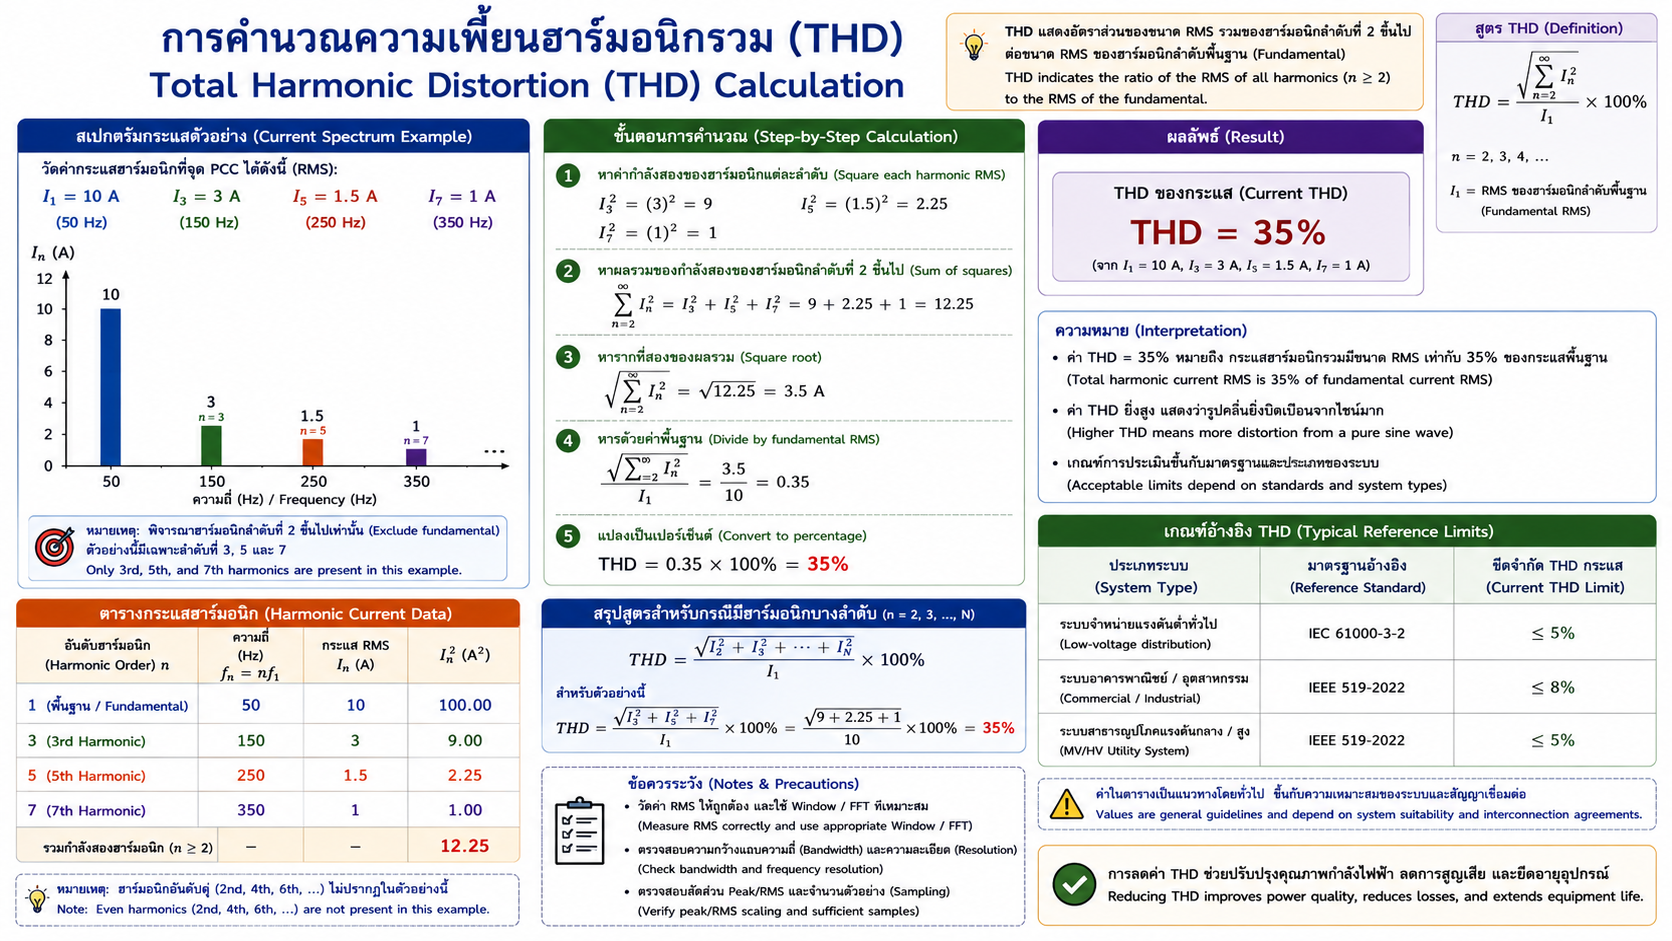
\includegraphics[width=0.8\textwidth]{images/chapter5/figure-06.png}
    \caption{การคำนวณ THD จากสเปกตรัม}
\end{figure}



\subsection{7.8 ผลกระทบของฮาร์มอนิกต่อระบบไฟฟ้า}

ฮาร์มอนิกไม่ได้ทำให้เกิดผลเสียเหมือนกันทุกระบบ ผลกระทบขึ้นกับขนาดฮาร์มอนิก อิมพีแดนซ์ของระบบ โครงสร้างสามเฟส อุปกรณ์ที่ต่อร่วม และตำแหน่งวัด การวิเคราะห์ที่ดีต้องพิจารณา “แหล่งกำเนิด–เส้นทาง–อุปกรณ์ที่รับผล” ร่วมกัน

\subsubsection{7.8.1 การสูญเสียและความร้อนเพิ่มขึ้น}

กระแส RMS ที่เพิ่มจากฮาร์มอนิกทำให้การสูญเสียแบบ $I^2R$ ในสายและขดลวดเพิ่มขึ้น

\[
P_{\mathrm{cu}}\approx I_{\mathrm{rms}}^2R
\]

อย่างไรก็ตาม ในความถี่สูง effective resistance อาจเพิ่มขึ้นจาก skin effect และ proximity effect ทำให้การสูญเสียจริงสูงกว่าการประมาณด้วย $R$ คงที่

\subsubsection{7.8.2 หม้อแปลง}

ฮาร์มอนิกสามารถเพิ่ม copper loss, eddy-current loss และความร้อนของหม้อแปลง โดยเฉพาะเมื่อมีกระแสฮาร์มอนิกความถี่สูง ในการใช้งานจริงจึงต้องพิจารณาการออกแบบและ derating ตามประเภทหม้อแปลงและข้อกำหนดที่เกี่ยวข้อง ไม่ควรใช้เพียงค่า THD เดียวตัดสิน

\subsubsection{7.8.3 สายนิวทรัลในระบบสามเฟสสี่สาย}

ฮาร์มอนิกลำดับที่เป็นสามเท่า เช่น 3, 9, 15 หรือ \textbf{triplen harmonics} มีลักษณะเฟสที่สามารถรวมกันในสายนิวทรัลแทนที่จะหักล้างเหมือน fundamental ของโหลดสามเฟสสมดุลบางกรณี จึงอาจทำให้กระแสนิวทรัลสูงอย่างไม่คาดคิดในระบบที่มีโหลดอิเล็กทรอนิกส์เฟสเดียวจำนวนมาก

\subsubsection{7.8.4 ตัวเก็บประจุและเรโซแนนซ์}

รีแอกแตนซ์ของตัวเก็บประจุลดลงเมื่อความถี่สูงขึ้น

\[
X_C=\frac{1}{2\pi fC}
\]

ขณะที่รีแอกแตนซ์ของตัวเหนี่ยวนำเพิ่มขึ้น

\[
X_L=2\pi fL
\]

เมื่อระบบมี L และ C อาจเกิด resonance ใกล้ความถี่ฮาร์มอนิก ทำให้กระแสหรือแรงดันบางความถี่ถูกขยาย ดังนั้นการติดตั้ง capacitor bank เพื่อแก้ power factor โดยไม่ประเมินฮาร์มอนิกและ resonance อาจสร้างปัญหาใหม่ได้

\subsubsection{7.8.5 มอเตอร์และเครื่องจักรไฟฟ้า}

ฮาร์มอนิกของแรงดันสามารถสร้างสนามแม่เหล็กและ torque pulsation เพิ่ม loss และ vibration ในเครื่องจักรไฟฟ้า ผลกระทบขึ้นกับ harmonic sequence และโครงสร้างของมอเตอร์

\subsubsection{7.8.6 อุปกรณ์ป้องกันและเครื่องมือวัด}

รูปคลื่นที่เพี้ยนอาจทำให้อุปกรณ์ที่ไม่ได้ออกแบบสำหรับ true RMS อ่านค่าไม่ถูกต้อง และอาจมีผลต่อการทำงานของอุปกรณ์ป้องกันบางชนิด การวัดเชิงคุณภาพกำลังจึงต้องใช้เครื่องมือและวิธีวัดที่เหมาะสม

\subsubsection{7.8.7 การรบกวนและการทำงานร่วมกันของอุปกรณ์}

ฮาร์มอนิกและองค์ประกอบความถี่สูงสามารถทำให้เกิดการรบกวนทางแม่เหล็กไฟฟ้าและปัญหาการทำงานร่วมกัน โดยเฉพาะเมื่อเส้นทางสายกำลังและสายสัญญาณอยู่ใกล้กัน แต่ต้องแยกปรากฏการณ์ low-frequency harmonics ออกจาก transient และ conducted/radiated EMI ที่มีช่วงความถี่ต่างกัน

\subsubsection{ตารางสรุปผลกระทบ}

\begin{table}[htbp]
    \centering
    \small
    \begin{tabularx}{\textwidth}{>{\raggedright\arraybackslash}p{0.16\textwidth} >{\raggedright\arraybackslash}X >{\raggedright\arraybackslash}X >{\raggedright\arraybackslash}X}
        \hline
        \textbf{อุปกรณ์/บริเวณ} & \textbf{กลไกหลัก} & \textbf{อาการที่อาจพบ} & \textbf{สิ่งที่ควรตรวจสอบ} \\
        \hline
        สายไฟ & RMS สูง, skin/proximity effect & ร้อน, สูญเสียเพิ่ม & RMS, harmonic spectrum, อุณหภูมิ \\
        สายนิวทรัล & triplen harmonics รวมกัน & กระแสนิวทรัลสูง & 3rd/9th/15th harmonic \\
        หม้อแปลง & copper/eddy loss & ความร้อน, อายุฉนวนลด & spectrum, loading, derating \\
        Capacitor bank & resonance / current amplification & กระแสสูง, fuse ขาด, capacitor เสีย & system impedance, resonant frequency \\
        มอเตอร์ & harmonic fields & loss, vibration, torque ripple & voltage spectrum, motor current \\
        เครื่องมือวัด & waveform sensitivity & ค่าอ่านคลาดเคลื่อน & true-RMS capability, bandwidth \\
        \hline
    \end{tabularx}
\end{table}

% [รูปที่ 7: ผลกระทบของฮาร์มอนิกต่อระบบไฟฟ้า]
% ประเภทภาพ: Technical Infographic
% ตำแหน่งที่แนะนำ: หัวข้อ 7.8
% วัตถุประสงค์การเรียนรู้: เชื่อมโยงฮาร์มอนิกกับอุปกรณ์ที่ได้รับผล
% คำอธิบายภาพ: single-line system แบบง่ายจาก PCC ไปยัง transformer, feeder, neutral, capacitor bank, motor และ electronic loads พร้อม callout ผลกระทบ
% องค์ประกอบที่ต้องมี: transformer, 3-phase 4-wire feeder, neutral, capacitor bank, motor, nonlinear loads
% ข้อความหรือป้ายกำกับ: “Heating”, “Neutral triplen current”, “Resonance”, “Torque ripple”, “Measurement error”
% ภาษาของป้ายกำกับ: ไทยและอังกฤษ
% สัดส่วนภาพ: 16:9
% Image Generation Prompt: Power-quality engineering infographic showing a simplified three-phase electrical distribution system with transformer, feeders, neutral conductor, capacitor bank, induction motor, and nonlinear electronic loads. Add callouts for harmonic effects: extra heating, triplen harmonic neutral current, capacitor resonance, motor torque ripple, and measurement error. White background, clean vector textbook style, bilingual Thai-English labels, 16:9.
% Alt Text: อินโฟกราฟิกระบบไฟฟ้าที่ชี้ผลของฮาร์มอนิกต่อสาย นิวทรัล หม้อแปลง capacitor bank มอเตอร์ และเครื่องมือวัด

\begin{figure}[htbp]
    \centering
    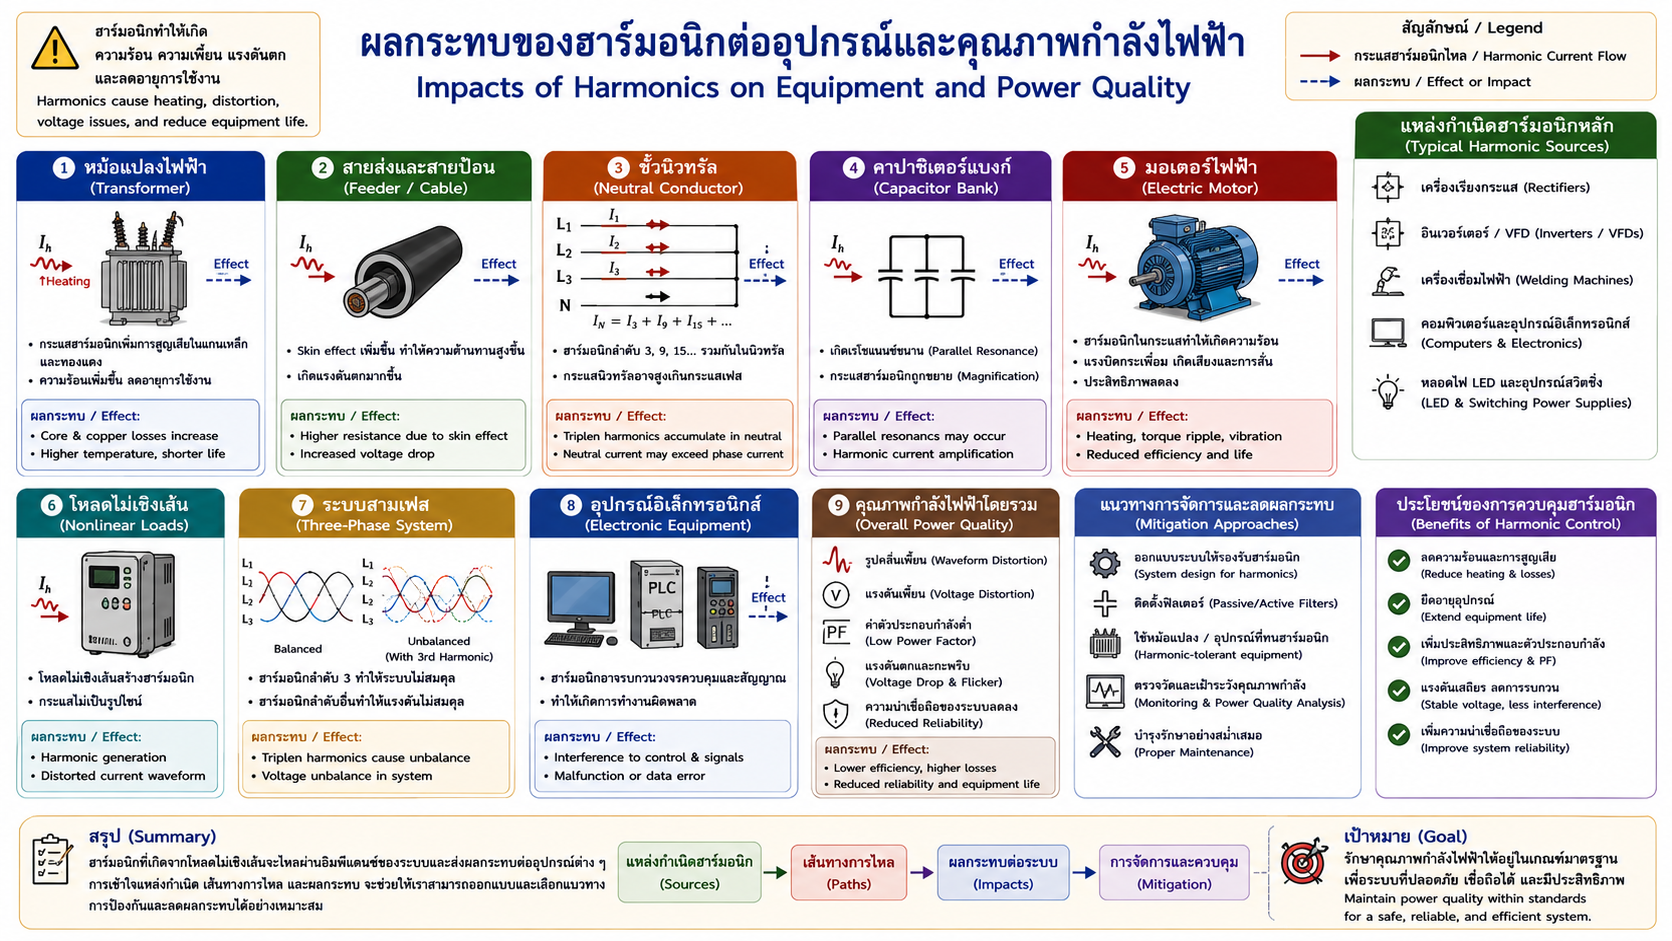
\includegraphics[width=0.8\textwidth]{images/chapter5/figure-07.png}
    \caption{ผลกระทบของฮาร์มอนิกต่อระบบไฟฟ้า}
\end{figure}



\subsection{7.9 การกรองสัญญาณและแนวคิดเบื้องต้นของฟิลเตอร์}

\subsubsection{7.9.1 เป้าหมายของการกรอง}

ฟิลเตอร์มีหน้าที่เลือกผ่านหรือลดทอนองค์ประกอบความถี่บางช่วง ในบริบทของฮาร์มอนิกอาจมีเป้าหมาย เช่น

\begin{itemize}
    \item รักษา fundamental 50 Hz แต่ลด 5th, 7th และฮาร์มอนิกลำดับสูง
    \item สร้างทางอิมพีแดนซ์ต่ำให้ฮาร์มอนิกเป้าหมายไหลผ่านแทนระบบ
    \item สร้างกระแสชดเชยที่มีขนาดเท่ากันแต่เฟสตรงข้ามกับฮาร์มอนิกของโหลด
\end{itemize}

\subsubsection{7.9.2 RC low-pass filter เพื่อเข้าใจแนวคิด}

วงจร RC low-pass มี transfer magnitude

\[
|H(j\omega)|=\frac{1}{\sqrt{1+(\omega RC)^2}}
\]

และความถี่ตัด

\[
f_c=\frac{1}{2\pi RC}
\]

\textbf{ที่มา:} ได้จาก voltage divider ระหว่าง $R$ และอิมพีแดนซ์ของตัวเก็บประจุ $Z_C=1/(j\omega C)$

\textbf{ความหมายทางกายภาพ:} ที่ความถี่ต่ำ capacitor มีอิมพีแดนซ์สูงและเอาต์พุตใกล้อินพุต ที่ความถี่สูง capacitor มีอิมพีแดนซ์ต่ำลงและสัญญาณเอาต์พุตถูกลดทอน

\textbf{ข้อจำกัด:} RC filter เหมาะสำหรับสัญญาณกำลังต่ำหรือวงจรสัญญาณ ไม่ควรนำค่าตัวอย่างไปต่อกับระบบไฟฟ้ากำลังโดยตรงโดยไม่ออกแบบพิกัดแรงดัน กระแส กำลัง และความปลอดภัย

\subsubsection{ตัวอย่างที่ 5: เปรียบเทียบการลดทอน fundamental กับ 5th harmonic}

\textbf{ตัวอย่างเพิ่มเติมเพื่อการเรียนรู้}

ออกแบบเชิงการเรียนรู้ให้ RC low-pass มี $f_c\approx100$ Hz โดยเลือก

\[
R=15.9\ \Omega,\qquad C=100\ \mu\mathrm{F}
\]

ตรวจสอบ

\[
f_c=\frac{1}{2\pi(15.9)(100\times10^{-6})}\approx100.1\ \text{Hz}
\]

สำหรับ 50 Hz

\[
|H(50)|=\frac{1}{\sqrt{1+(50/100.1)^2}}\approx0.895
\]

สำหรับ 5th harmonic ที่ 250 Hz

\[
|H(250)|=\frac{1}{\sqrt{1+(250/100.1)^2}}\approx0.372
\]

\textbf{การแปลความหมาย:} filter นี้ลด fundamental เหลือประมาณ 89.5\% แต่ลด 5th harmonic เหลือประมาณ 37.2\% จึงแสดงหลักการ “ความถี่สูงถูกลดทอนมากกว่า” แต่ยังไม่ใช่การออกแบบ power harmonic filter ที่เหมาะสม เพราะ fundamental ถูกลดทอนมากเกินไปและไม่ได้พิจารณาพิกัดกำลัง

\subsubsection{7.9.3 LC tuned filter}

วงจร L-C มีความถี่เรโซแนนซ์เชิงอุดมคติ

\[
f_r=\frac{1}{2\pi\sqrt{LC}}
\]

ถ้าต้องการ tune ใกล้ 5th harmonic ของ 50 Hz จะมี

\[
f_r\approx250\ \text{Hz}
\]

ตัวอย่าง หากเลือก $C=20\ \mu\mathrm{F}$

\[
L=\frac{1}{(2\pi f_r)^2C}
\]

\[
L\approx20.3\ \text{mH}
\]

ในระบบจริงต้องมีการพิจารณา damping, component tolerance, reactive power, system impedance, detuning และ resonance กับระบบ จึงไม่ควรใช้สมการอุดมคติเพียงสมการเดียวเพื่อสร้างฟิลเตอร์กำลังจริง

\subsubsection{7.9.4 Passive harmonic filter}

ฟิลเตอร์พาสซีฟในระบบกำลังอาจใช้แขนง RLC ที่ tune ใกล้ฮาร์มอนิกเป้าหมายเพื่อสร้างเส้นทางอิมพีแดนซ์ต่ำให้กระแสฮาร์มอนิก หรือใช้ high-pass configuration สำหรับฮาร์มอนิกลำดับสูง ข้อดีคือโครงสร้างไม่ซับซ้อนและไม่ต้องมีวงจรควบคุมความเร็วสูง แต่การทำงานขึ้นกับอิมพีแดนซ์ของระบบและอาจมีปัญหา resonance หรือ detuning

\subsubsection{7.9.5 Active power filter}

Active power filter วัดกระแสหรือแรงดันของระบบ ประเมินส่วนที่ต้องการชดเชย แล้วใช้อุปกรณ์อิเล็กทรอนิกส์กำลังสร้างกระแสชดเชย ตัวอย่างแนวคิด

\[
i_s(t)=i_L(t)-i_c(t)
\]

ถ้า $i_c(t)$ ถูกสร้างให้ใกล้เคียงส่วนฮาร์มอนิกของโหลด กระแสด้านแหล่งจ่าย $i_s(t)$ จะเข้าใกล้รูปคลื่น fundamental มากขึ้น

\subsubsection{7.9.6 เปรียบเทียบแนวทางกรอง}

\begin{table}[htbp]
    \centering
    \small
    \begin{tabularx}{\textwidth}{>{\raggedright\arraybackslash}p{0.20\textwidth} >{\raggedright\arraybackslash}X >{\raggedright\arraybackslash}X >{\raggedright\arraybackslash}X}
        \hline
        \textbf{แนวทาง} & \textbf{หลักการ} & \textbf{ข้อดี} & \textbf{ข้อจำกัด} \\
        \hline
        RC/LC low-pass & ลดความถี่สูง & เข้าใจง่าย & อาจลด fundamental, ต้องออกแบบพิกัด \\
        Tuned passive filter & สร้าง low impedance ที่ฮาร์มอนิกเป้าหมาย & โครงสร้างไม่ซับซ้อน & detuning/resonance, ไวต่อระบบ \\
        High-pass passive & ระบายฮาร์มอนิกลำดับสูง & ครอบคลุมช่วงกว้างขึ้น & loss และการเลือกค่า RLC \\
        Active power filter & ฉีดกระแสชดเชย & ปรับตามโหลดได้ & ราคาและระบบควบคุมซับซ้อน \\
        \hline
    \end{tabularx}
\end{table}

% [รูปที่ 8: เปรียบเทียบฟิลเตอร์พาสซีฟและแอ็กทีฟสำหรับฮาร์มอนิก]
% ประเภทภาพ: Block Diagram / Technical Illustration
% ตำแหน่งที่แนะนำ: หลังหัวข้อ 7.9.6
% วัตถุประสงค์การเรียนรู้: เปรียบเทียบกลไกการลดฮาร์มอนิกสองแนวทาง
% คำอธิบายภาพ: ซ้ายเป็น shunt passive tuned filter ต่อที่ PCC ขวาเป็น active filter วัดโหลดและฉีด compensating current
% องค์ประกอบที่ต้องมี: source, PCC, nonlinear load, RLC branch, current sensor, active converter, compensation current arrow
% ข้อความหรือป้ายกำกับ: “Passive tuned path”, “Active compensation”, “Harmonic current”
% ภาษาของป้ายกำกับ: ไทยและอังกฤษ
% สัดส่วนภาพ: 16:9
% Image Generation Prompt: Side-by-side electrical engineering diagram comparing passive and active harmonic filtering. Left: AC source, PCC, nonlinear load, and a shunt tuned RLC harmonic filter providing a low-impedance path for harmonic current. Right: AC source, PCC, nonlinear load, current sensor, active power filter converter injecting compensating current opposite to the harmonic current. White background, bilingual Thai-English labels, clean vector textbook style, 16:9.
% Alt Text: แผนภาพเปรียบเทียบ passive filter ที่ระบายฮาร์มอนิกผ่านวงจร RLC กับ active filter ที่ฉีดกระแสชดเชย

\begin{figure}[htbp]
    \centering
    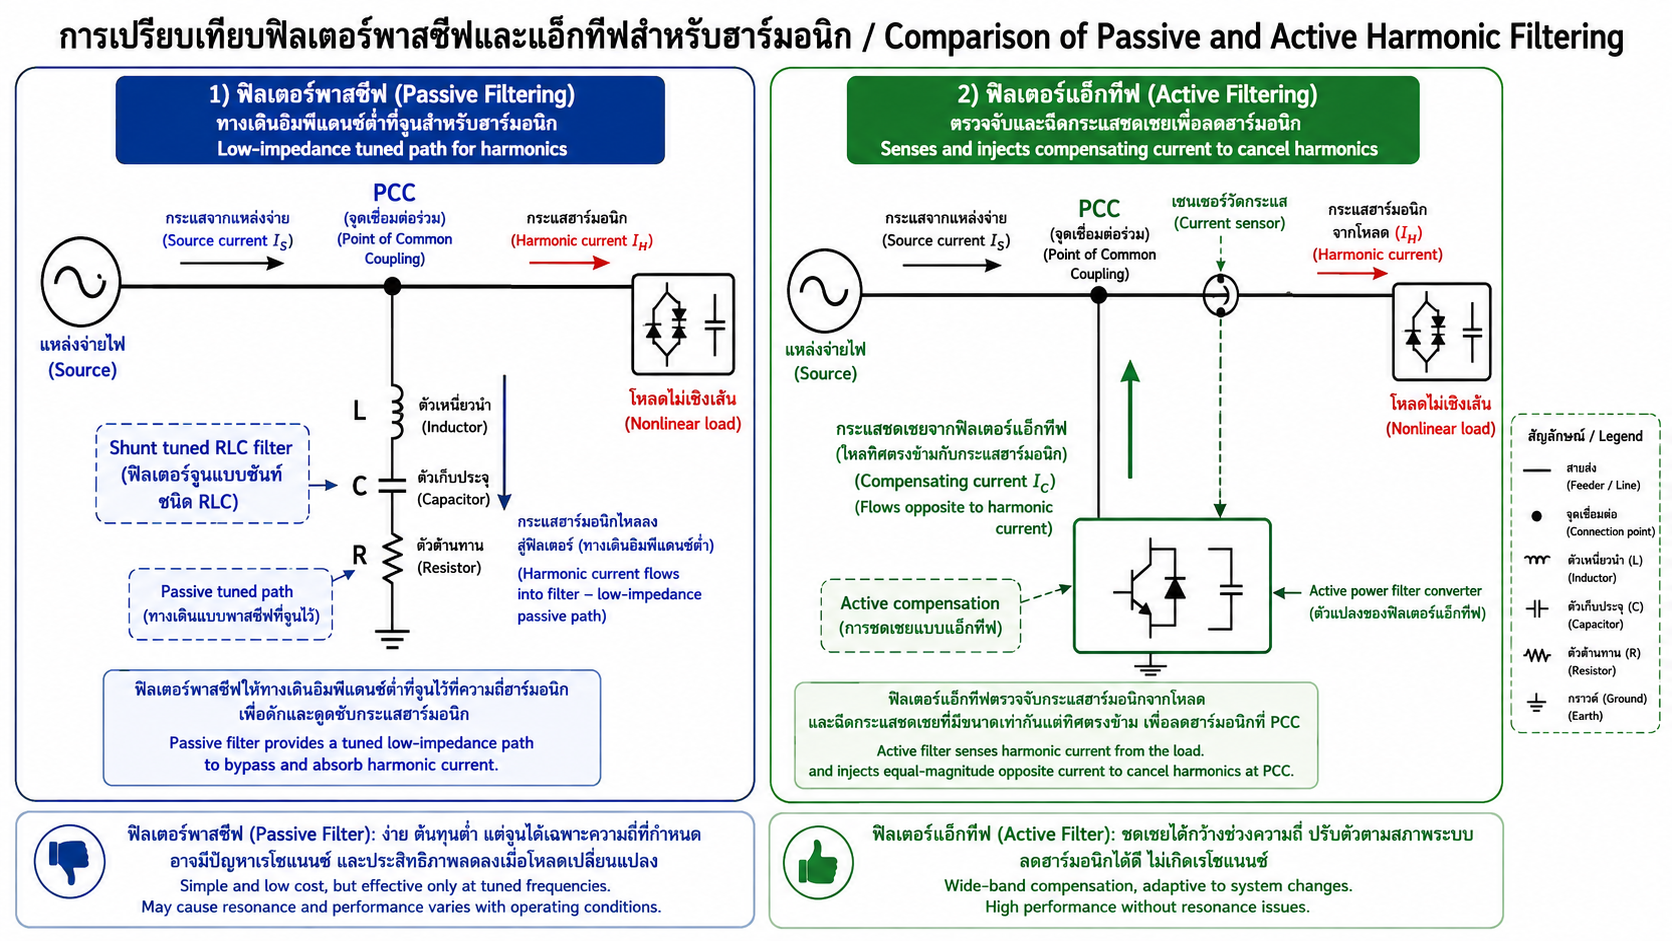
\includegraphics[width=0.8\textwidth]{images/chapter5/figure-08.png}
    \caption{เปรียบเทียบฟิลเตอร์พาสซีฟและแอ็กทีฟสำหรับฮาร์มอนิก}
\end{figure}



\subsection{7.10 การใช้โปรแกรมคำนวณวิเคราะห์รูปคลื่นไฟฟ้า}

หัวข้อนี้ใช้โปรแกรมเป็นเครื่องมือ \textbf{ตรวจสอบแนวคิดคณิตศาสตร์} ไม่ใช่แทนที่ความเข้าใจ ผู้เรียนควรรู้ก่อนว่า FFT ให้ข้อมูลอะไร ขนาดสเปกตรัมถูก normalize อย่างไร และความละเอียดความถี่สัมพันธ์กับเวลาบันทึกสัญญาณอย่างไร

\subsubsection{7.10.1 จากสัญญาณต่อเนื่องสู่ข้อมูลตัวอย่าง}

ให้ sample สัญญาณด้วยอัตรา

\[
f_s=\frac{1}{\Delta t}
\]

ถ้ามีตัวอย่าง $N$ จุด ระยะเวลาบันทึกประมาณ

\[
T_{\mathrm{obs}}=\frac{N}{f_s}
\]

และ frequency-bin spacing ของ DFT คือ

\[
\Delta f=\frac{f_s}{N}=\frac{1}{T_{\mathrm{obs}}}
\]

ดังนั้น หากต้องการแยกความถี่ที่อยู่ใกล้กันมาก ต้องเพิ่มเวลาบันทึก ไม่ใช่เพียงเพิ่ม sampling rate อย่างเดียว

\subsubsection{7.10.2 Sampling และ Nyquist consideration}

ความถี่สูงสุดที่แทนได้โดยไม่เกิด aliasing ภายใต้เงื่อนไข sampling อุดมคติคือ

\[
f_{\mathrm{Nyquist}}=\frac{f_s}{2}
\]

ในระบบวัดจริงยังต้องพิจารณา anti-alias filter, bandwidth ของ sensor และเครื่องมือวัด

\subsubsection{7.10.3 Spectral leakage}

ถ้าช่วงข้อมูลที่เลือกไม่ประกอบด้วยจำนวนคาบที่เหมาะสม พลังงานของไซน์หนึ่งความถี่อาจกระจายไปหลาย frequency bins เรียกว่า \textbf{spectral leakage} การใช้ window ช่วยลด leakage บางลักษณะ แต่ทำให้ main lobe กว้างขึ้นและมีผลต่อ amplitude estimation ดังนั้นผู้เรียนควรเรียนรู้ว่า “FFT plot” ขึ้นกับวิธีเก็บข้อมูลและประมวลผล ไม่ใช่ความจริงที่ไม่ต้องตีความ

\subsubsection{7.10.4 ตัวอย่าง Python: สร้างรูปคลื่นและคำนวณ FFT}

ตัวอย่างต่อไปนี้ใช้ NumPy และ Matplotlib โดยสร้างสัญญาณ 50 Hz ที่มี 3rd และ 5th harmonic

\begin{verbatim}
import numpy as np
import matplotlib.pyplot as plt

fs = 10000.0          # sampling frequency, Hz
Tobs = 0.2            # observation time, s
N = int(fs * Tobs)
t = np.arange(N) / fs

# RMS amplitudes
I1 = 10.0
I3 = 3.0
I5 = 1.5

# Convert RMS amplitude to peak with sqrt(2)
i = (np.sqrt(2)*I1*np.sin(2*np.pi*50*t)
     + np.sqrt(2)*I3*np.sin(2*np.pi*150*t - np.deg2rad(20))
     + np.sqrt(2)*I5*np.sin(2*np.pi*250*t + np.deg2rad(30)))

# One-sided FFT for real-valued input
Y = np.fft.rfft(i)
f = np.fft.rfftfreq(N, d=1/fs)

# Convert two-sided-equivalent FFT coefficient to peak amplitude
Apeak = 2*np.abs(Y) / N
Apeak[0] = np.abs(Y[0]) / N

# Convert sinusoidal peak amplitudes to RMS
Arms = Apeak / np.sqrt(2)
Arms[0] = Apeak[0]   # DC RMS equals DC magnitude

plt.figure()
plt.plot(t*1000, i)
plt.xlim(0, 40)
plt.xlabel('Time (ms)')
plt.ylabel('Current (A)')
plt.title('Distorted current waveform')
plt.grid(True)

plt.figure()
mask = f <= 500
plt.stem(f[mask], Arms[mask])
plt.xlabel('Frequency (Hz)')
plt.ylabel('RMS magnitude (A)')
plt.title('One-sided RMS spectrum')
plt.grid(True)
plt.show()
\end{verbatim}

\textbf{สิ่งที่ควรสังเกต}

\begin{itemize}
    \item $f_s=10$ kHz
    \item $T_{\mathrm{obs}}=0.2$ s
    \item $N=2000$
    \item ความละเอียดความถี่
\end{itemize}

\[
\Delta f=\frac{10000}{2000}=5\ \text{Hz}
\]

ดังนั้น 50, 150 และ 250 Hz อยู่ตรงกับ frequency bins พอดีในตัวอย่างนี้ ทำให้การอ่านแอมพลิจูดตรงไปตรงมา

\subsubsection{7.10.5 คำนวณ THD จากค่าฮาร์มอนิกใน Python}

ถ้าทราบ RMS harmonic magnitudes แล้ว สามารถคำนวณโดยตรง

\begin{verbatim}
I1 = 10.0
harmonics = np.array([3.0, 1.5, 1.0])
thd = np.sqrt(np.sum(harmonics**2)) / I1
print(f"THD = {100*thd:.2f}%")
\end{verbatim}

ผลที่คาดหวังคือ

\begin{verbatim}
THD = 35.00%
\end{verbatim}

\subsubsection{7.10.6 ตัวอย่าง MATLAB/Octave แนวคิดเดียวกัน}

\begin{verbatim}
fs = 10000;
Tobs = 0.2;
N = fs*Tobs;
t = (0:N-1)/fs;

i = sqrt(2)*10*sin(2*pi*50*t) ...
  + sqrt(2)*3*sin(2*pi*150*t - deg2rad(20)) ...
  + sqrt(2)*1.5*sin(2*pi*250*t + deg2rad(30));

Y = fft(i);
f = (0:N-1)*(fs/N);

Apeak = 2*abs(Y)/N;
Arms = Apeak/sqrt(2);

idx = f <= 500;
stem(f(idx), Arms(idx));
xlabel('Frequency (Hz)');
ylabel('Approx. RMS magnitude (A)');
grid on;
\end{verbatim}

\textbf{หมายเหตุ:} ในการใช้งานจริงต้องจัดการ one-sided spectrum, DC, Nyquist bin, window scaling และ normalization อย่างถูกต้อง การใช้ฟังก์ชันสำเร็จรูปสำหรับ THD อาจใช้วิธีประเมินสเปกตรัมหรือจำนวนฮาร์มอนิกต่างจากสูตรที่คำนวณด้วยมือ ผู้เรียนควรอ่านเอกสารฟังก์ชันของเวอร์ชันซอฟต์แวร์ที่ใช้และระบุวิธีคำนวณในรายงาน

\subsubsection{7.10.7 กระบวนการวิเคราะห์ FFT ที่แนะนำ}

\begin{enumerate}
    \item ระบุชนิดสัญญาณและหน่วย
    \item ทราบหรือประมาณ $f_0$
    \item เลือก $f_s$ ให้สูงพอสำหรับความถี่สูงสุดที่สนใจ
    \item เลือกช่วงข้อมูลที่เป็น steady state
    \item ตรวจสอบจำนวนคาบในช่วงข้อมูล
    \item เลือก window หากจำเป็น
    \item คำนวณ FFT/DFT
    \item normalize amplitude อย่างถูกต้อง
    \item แปลง peak $\leftrightarrow$ RMS ให้ชัดเจน
    \item ระบุ harmonic bins หรือใช้ peak detection อย่างมีหลักเกณฑ์
    \item คำนวณ THD
    \item เปรียบเทียบผลกับการคำนวณเชิงทฤษฎีหรือข้อมูลเครื่องมือวัด
\end{enumerate}

% [รูปที่ 9: ขั้นตอนการวิเคราะห์ฮาร์มอนิกด้วย FFT]
% ประเภทภาพ: Flowchart
% ตำแหน่งที่แนะนำ: หลังหัวข้อ 7.10.7
% วัตถุประสงค์การเรียนรู้: ให้ผู้เรียนเห็น workflow ที่ถูกต้องตั้งแต่การเก็บข้อมูลถึงการตีความ THD
% คำอธิบายภาพ: flowchart 8–10 ขั้น จาก waveform acquisition → sampling → steady-state window → FFT → normalization → spectrum → harmonic extraction → RMS/THD → validation
% องค์ประกอบที่ต้องมี: sampling rate, observation time, window, FFT, frequency bins, RMS, THD, validation
% ข้อความหรือป้ายกำกับ: “Avoid aliasing”, “Check leakage”, “Peak or RMS?”, “Validate with theory”
% ภาษาของป้ายกำกับ: ไทยและอังกฤษ
% สัดส่วนภาพ: 16:9
% Image Generation Prompt: Engineering education flowchart for harmonic analysis using FFT. Steps: acquire waveform, choose sampling frequency, select steady-state observation window, check number of cycles, apply window if needed, compute FFT, normalize one-sided spectrum, convert amplitude to RMS, identify harmonic orders, calculate THD, validate against theory. Include warning callouts for aliasing, spectral leakage, and peak-vs-RMS scaling. White background, bilingual Thai-English labels, clean vector style, 16:9.
% Alt Text: ผังงานวิเคราะห์ FFT ตั้งแต่การเก็บข้อมูล เลือก sampling และ window ไปจนถึงการหาสเปกตรัม RMS และ THD พร้อมตรวจสอบ aliasing และ leakage

\begin{figure}[htbp]
    \centering
    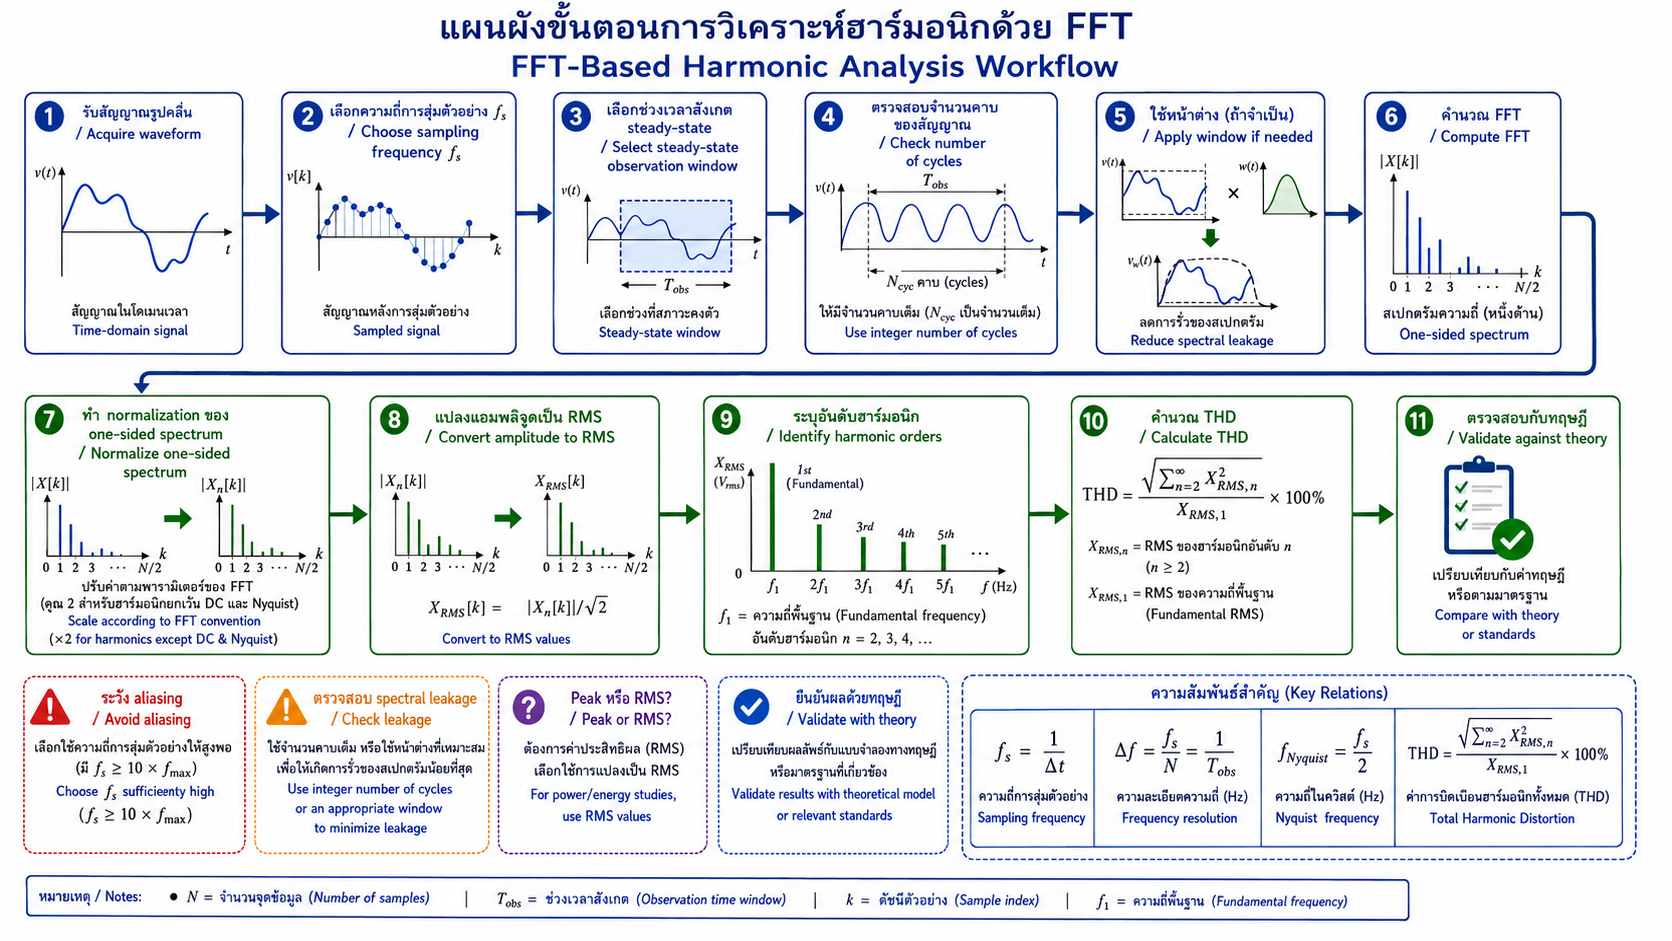
\includegraphics[width=0.8\textwidth]{images/chapter5/figure-09.png}
    \caption{ขั้นตอนการวิเคราะห์ฮาร์มอนิกด้วย FFT}
\end{figure}



\subsection{7.11 ตัวอย่างโจทย์และการคำนวณแบบเป็นขั้นตอน}

หัวข้อนี้รวบรวมตัวอย่างประยุกต์ที่เชื่อม RMS, THD, กำลัง และฟิลเตอร์เข้าด้วยกัน

\subsubsection{ตัวอย่างที่ 6: จาก THD ไปสู่กระแส RMS และ true PF}

\textbf{ตัวอย่างเพิ่มเติมเพื่อการเรียนรู้}

โหลดเฟสเดียวรับแรงดันไซน์บริสุทธิ์ 230 V RMS ดึง fundamental current 12 A RMS มี $\mathrm{THD}_I=40\%$ และ displacement factor ที่ fundamental เท่ากับ 0.95 จงหา

\begin{enumerate}
    \item กระแส RMS รวม
    \item กำลังจริง
    \item apparent power
    \item true PF
\end{enumerate}

\textbf{ขั้นที่ 1 กำหนดตัวแปร}

\[
\begin{aligned}
    V_1=230\ \text{V},\quad I_1=12\ \text{A},\quad \mathrm{THD}_I=0.40, \\
    \quad \cos\phi_1=0.95
\end{aligned}
\]

\textbf{ขั้นที่ 2 หา RMS รวม}

\[
I_{\mathrm{rms}}=I_1\sqrt{1+\mathrm{THD}_I^2}
\]

\[
=12\sqrt{1+0.4^2}
\]

\[
=12\sqrt{1.16}=12.92\ \text{A}
\]

\textbf{ขั้นที่ 3 หากำลังจริง}

แรงดันเป็นไซน์บริสุทธิ์ จึงมีเพียง fundamental voltage

\[
P=V_1I_1\cos\phi_1
\]

\[
=230(12)(0.95)=2622\ \text{W}
\]

\textbf{ขั้นที่ 4 หา apparent power}

\[
S=V_{\mathrm{rms}}I_{\mathrm{rms}}=230(12.92)=2971.6\ \text{VA}
\]

\textbf{ขั้นที่ 5 หา true PF}

\[
PF=\frac{2622}{2971.6}=0.882
\]

\textbf{ขั้นที่ 6 ตรวจสอบทางเลือก}

\[
\begin{aligned}
    \frac{I_1}{I_{\mathrm{rms}}}\cos\phi_1 \\
    =\frac{12}{12.92}(0.95)\approx0.882
\end{aligned}
\]

ตรงกัน

\textbf{คำตอบ}

\[
\boxed{I_{\mathrm{rms}}\approx12.92\ \text{A},\quad P\approx2.622\ \text{kW},\quad S\approx2.972\ \text{kVA},\quad PF\approx0.882}
\]

\subsubsection{ตัวอย่างที่ 7: วิเคราะห์ว่าฮาร์มอนิกลำดับใดควรให้ความสำคัญ}

\textbf{ตัวอย่างเพิ่มเติมเพื่อการเรียนรู้}

วัดกระแสโหลดได้

\begin{table}[htbp]
    \centering
    \begin{tabular}{r r}
        \hline
        \textbf{Harmonic} & \textbf{RMS current} \\
        \hline
        1 & 20 A \\
        3 & 8 A \\
        5 & 2 A \\
        7 & 1.5 A \\
        9 & 3 A \\
        \hline
    \end{tabular}
\end{table}

จงจัดลำดับความสำคัญของฮาร์มอนิกสำหรับการวิเคราะห์

\textbf{ขั้นที่ 1 คำนวณสัดส่วนเทียบ fundamental}

\[
I_3/I_1=8/20=40\%
\]

\[
I_5/I_1=10\%,\quad I_7/I_1=7.5\%,\quad I_9/I_1=15\%
\]

\textbf{ขั้นที่ 2 พิจารณาบริบท} \\
ถ้าเป็นระบบสามเฟสสี่สายที่มีโหลดเฟสเดียวจำนวนมาก 3rd และ 9th เป็น triplen harmonics จึงควรตรวจสอบสายนิวทรัลเป็นพิเศษ

\textbf{ขั้นที่ 3 สรุป} \\
3rd harmonic มีขนาดสูงสุดและมีนัยสำคัญทั้งด้าน THD และ neutral current ส่วน 9th แม้ต่ำกว่า 5th ในบางระบบทั่วไป แต่มีลักษณะ triplen จึงควรให้ความสำคัญเชิงโครงสร้างระบบ

\textbf{ข้อสังเกต:} การจัดลำดับจาก “ขนาด” เพียงอย่างเดียวไม่พอ ต้องพิจารณาคุณสมบัติของ harmonic order และอุปกรณ์ในระบบด้วย

\subsubsection{ตัวอย่างที่ 8: ประเมิน tuned frequency ของฟิลเตอร์}

\textbf{ตัวอย่างเพิ่มเติมเพื่อการเรียนรู้}

ระบบ 50 Hz พบ 5th harmonic เด่น ต้องการใช้แบบจำลอง LC เพื่อเรียนรู้การ tune ใกล้ 250 Hz หาก $C=20\ \mu$F จงหา $L$

\textbf{ขั้นที่ 1 ความถี่เป้าหมาย}

\[
f_5=5f_0=5(50)=250\ \text{Hz}
\]

\textbf{ขั้นที่ 2 ใช้สมการ resonance}

\[
f_r=\frac{1}{2\pi\sqrt{LC}}
\]

จัดรูป

\[
L=\frac{1}{(2\pi f_r)^2C}
\]

\textbf{ขั้นที่ 3 แทนค่า}

\[
L=\frac{1}{(2\pi\times250)^2(20\times10^{-6})}
\]

\[
L\approx0.0203\ \text{H}=20.3\ \text{mH}
\]

\textbf{ขั้นที่ 4 แปลความหมายและข้อจำกัด} \\
ค่านี้เป็นค่าทางทฤษฎีของ LC อุดมคติ การออกแบบฟิลเตอร์จริงต้องพิจารณา R, Q-factor, tolerance, detuning, reactive power และ system resonance

\textbf{คำตอบ}

\[
\boxed{L\approx20.3\ \text{mH}}
\]



\subsection{7.12 กิจกรรมการเรียนรู้และแบบฝึกหัดท้ายบท}

รายละเอียดกิจกรรมและแบบฝึกหัดฉบับเต็มอยู่ในหัวข้อ 11–12 ของบท เพื่อให้สอดคล้องกับรูปแบบมาตรฐานของเอกสารประกอบการสอนทั้งรายวิชา โดยกิจกรรมจะเน้นการอ่านสเปกตรัม การคำนวณ RMS/THD การเชื่อมโยงฮาร์มอนิกกับ power quality และการตรวจสอบผลด้วยโปรแกรมคำนวณ



\subsection{8. ความเข้าใจผิดที่พบบ่อย}

\subsubsection{8.1 “THD ต่ำ แปลว่ารูปคลื่นดีทุกด้าน”}

ไม่ถูกต้อง THD วัดเฉพาะฮาร์มอนิกเทียบ fundamental และไม่บอก transient, flicker, unbalance, interharmonics หรือเฟสขององค์ประกอบ ความสมบูรณ์ของ power quality จึงต้องใช้พารามิเตอร์หลายชนิด

\subsubsection{8.2 “ฮาร์มอนิกลำดับที่ 5 คือความถี่ 5 Hz”}

ไม่ถูกต้อง harmonic order เป็น \textbf{ตัวคูณของ fundamental} ถ้า $f_0=50$ Hz, 5th harmonic คือ 250 Hz

\subsubsection{8.3 “RMS ของหลายฮาร์มอนิกบวกกันตรง ๆ”}

ไม่ถูกต้อง ต้องใช้ root-sum-square

\[
X_{\mathrm{rms}}=\sqrt{\sum X_n^2}
\]

เมื่อ $X_n$ เป็น RMS ขององค์ประกอบออร์โทโกนัล

\subsubsection[8.4 ถ้า cos phi1 = 1 ตัวประกอบกำลังรวมต้องเป็น 1]{8.4 “ถ้า $\cos\phi_1=1$ ตัวประกอบกำลังรวมต้องเป็น 1”}

ไม่จำเป็น ถ้ากระแสมีฮาร์มอนิก true PF อาจต่ำกว่า 1 เพราะ $I_{\mathrm{rms}}>I_1$

\subsubsection{8.5 “FFT กับ Fourier series เป็นสิ่งเดียวกันทุกกรณี”}

Fourier series เป็นการแทนสัญญาณเป็นคาบด้วยองค์ประกอบความถี่แบบไม่ต่อเนื่อง ส่วน DFT/FFT เป็นวิธีคำนวณเชิงตัวเลขจากข้อมูล sampled ที่มีจำนวนจุดจำกัด การเลือก sampling, observation window และ scaling มีผลต่อผลลัพธ์

\subsubsection{8.6 “ถ้า FFT มี peak หลายจุด แสดงว่าระบบมีฮาร์มอนิกจริงทั้งหมด”}

ไม่เสมอ อาจเกิด spectral leakage, noise, modulation, interharmonics, aliasing หรือ artifacts จากการวัด ต้องตรวจสอบว่าความถี่เป็นจำนวนเต็มเท่าของ $f_0$ และพิจารณาวิธีวัด

\subsubsection{8.7 “ฟิลเตอร์ที่ tune ตรงฮาร์มอนิกเป๊ะที่สุดย่อมดีที่สุด”}

ในระบบจริงค่า L, C เปลี่ยนตาม tolerance และอุณหภูมิ อีกทั้ง system impedance เปลี่ยนได้ การ tune แบบอุดมคติอาจเกิด resonance ที่ไม่ต้องการ จึงต้องออกแบบเผื่อ detuning และ damping ตามหลักวิศวกรรม

\subsubsection{8.8 “ค่า THD จากซอฟต์แวร์ทุกโปรแกรมต้องตรงกันทันที”}

ไม่เสมอ เพราะซอฟต์แวร์อาจใช้จำนวนฮาร์มอนิก, window, periodogram, bandwidth, normalization และนิยามตัวหารต่างกัน ต้องอ่าน documentation และระบุวิธีวิเคราะห์ให้ชัดเจน



\subsection{9. การประยุกต์ใช้ในงานจริง}

\subsubsection{9.1 แหล่งจ่ายไฟแบบสวิตชิ่ง}

วงจร rectifier-capacitor input อาจดึงกระแสเป็นพัลส์ใกล้ยอดของแรงดัน ทำให้กระแสมีฮาร์มอนิกหลายลำดับ การวิเคราะห์ Fourier ช่วยบอกว่าความถี่ใดเป็นส่วนสำคัญและช่วยประเมิน RMS current ของสายและอุปกรณ์

\subsubsection{9.2 Variable-frequency drive และ inverter}

อุปกรณ์สวิตชิ่งสร้าง waveform ที่มีองค์ประกอบหลายความถี่ ทั้งด้าน input และ output การแยก fundamental ออกจาก harmonic และ switching components ช่วยในการเลือก filter, motor และเครื่องมือวัด อย่างไรก็ตาม switching-frequency components อาจอยู่นอกขอบเขต harmonic power-frequency แบบคลาสสิก และต้องใช้ bandwidth/EMC analysis เพิ่มเติม

\subsubsection{9.3 ระบบสามเฟสในอาคารที่มีโหลด IT จำนวนมาก}

คอมพิวเตอร์ LED driver และ electronic power supply แบบเฟสเดียวจำนวนมากอาจสร้าง triplen harmonics ทำให้ neutral current สูง การดูเพียง phase RMS โดยไม่ดู harmonic spectrum อาจพลาดปัญหานี้

\subsubsection{9.4 ระบบพลังงานหมุนเวียนและอินเวอร์เตอร์}

PV inverter และ battery inverter ใช้ power electronics การประเมินคุณภาพกระแสและแรงดันจึงต้องพิจารณาฮาร์มอนิกที่ PCC ร่วมกับเงื่อนไข grid connection ตามมาตรฐานและข้อกำหนดท้องถิ่น

\subsubsection{9.5 เครื่องมือวัด power quality}

เครื่องมือวัดสมัยใหม่มักรายงาน RMS, harmonic spectrum, THD, unbalance และ event ต่าง ๆ ผู้ใช้งานต้องเข้าใจว่าค่าที่เครื่องมือแสดงมาจากการประมวลผลสัญญาณอย่างไร เพื่อไม่ตีความตัวเลขผิดบริบท

\subsubsection{9.6 การตรวจสอบปัญหาความร้อนผิดปกติ}

หากสายหรือหม้อแปลงร้อนเกินคาดทั้งที่ fundamental current ดูไม่สูง การวัด true RMS และ harmonic spectrum อาจเผยให้เห็นฮาร์มอนิกที่เพิ่ม loss และ neutral loading ได้



\subsection{10. สรุปท้ายบท}

\begin{enumerate}
    \item รูปคลื่นไฟฟ้าเป็นคาบที่ไม่เป็นไซน์สามารถแยกเป็น DC และฮาร์มอนิกด้วยอนุกรมฟูเรียร์
    \item ฮาร์มอนิกลำดับที่ $n$ มีความถี่ $f_n=nf_0$
    \item รูปคลื่นสี่เหลี่ยมมี odd harmonics ลดลงประมาณ $1/n$ ส่วนรูปสามเหลี่ยมลดลงเร็วกว่า คือประมาณ $1/n^2$
    \item ค่า RMS ของสัญญาณทั่วไปต้องมาจากนิยามกำลังสองเฉลี่ย หรือคำนวณจากองค์ประกอบฟูเรียร์ด้วย root-sum-square
    \item กำลังเฉลี่ยของรูปคลื่นไม่เป็นไซน์คำนวณจาก $P=(1/T)\int vi\,dt$ และในโดเมนฮาร์มอนิก องค์ประกอบที่มีลำดับเดียวกันมีส่วนต่อกำลังเฉลี่ย
    \item true power factor อาจต่ำกว่า displacement factor เมื่อกระแสมี distortion
    \item THD เป็นอัตราส่วน RMS ของฮาร์มอนิกต่อ fundamental แต่ไม่แทนข้อมูลสเปกตรัมทั้งหมดและไม่ใช่ตัวชี้วัด power quality เพียงตัวเดียว
    \item ฮาร์มอนิกอาจเพิ่มความร้อน การสูญเสีย neutral current resonance และผลกระทบต่อมอเตอร์หรือเครื่องมือวัด
    \item ฟิลเตอร์พาสซีฟและแอ็กทีฟลดฮาร์มอนิกด้วยกลไกต่างกัน และการออกแบบจริงต้องพิจารณา system impedance และพิกัดอุปกรณ์
    \item FFT เป็นเครื่องมือสำคัญสำหรับข้อมูล sampled แต่ต้องควบคุม sampling rate, observation time, leakage, window และ amplitude scaling
\end{enumerate}

\subsubsection{สมการหลักของบท}

\[
f_n=nf_0
\]

\[
X_{\mathrm{rms}}=\sqrt{\frac{1}{T}\int_T x^2(t)dt}
\]

\[
X_{\mathrm{rms}}^2=X_{\mathrm{DC}}^2+\sum_{n=1}^{\infty}X_{n,\mathrm{rms}}^2
\]

\[
P=\frac{1}{T}\int_T v(t)i(t)dt
\]

\[
P=V_{\mathrm{DC}}I_{\mathrm{DC}}+\sum_{n=1}^{\infty}V_nI_n\cos\phi_n
\]

\[
S=V_{\mathrm{rms}}I_{\mathrm{rms}}
\]

\[
PF=\frac{P}{S}
\]

\[
\mathrm{THD}_X=\frac{\sqrt{\sum_{n=2}^{\infty}X_n^2}}{X_1}\times100\%
\]

\[
f_c=\frac{1}{2\pi RC}
\]

\[
f_r=\frac{1}{2\pi\sqrt{LC}}
\]

\[
\Delta f=\frac{f_s}{N}=\frac{1}{T_{\mathrm{obs}}}
\]



\subsection{11. คำถามทบทวน}

\begin{enumerate}
    \item อธิบายความแตกต่างระหว่าง \textbf{fundamental frequency}, \textbf{harmonic order} และ \textbf{harmonic frequency} พร้อมยกตัวอย่างสำหรับระบบ 50 Hz
    \item เพราะเหตุใดรูปคลื่นสี่เหลี่ยมจึงมีฮาร์มอนิกลำดับสูงเด่นกว่ารูปคลื่นสามเหลี่ยม เมื่อพิจารณาการลดลงของ Fourier coefficients
    \item ค่าเฉลี่ยของรูปคลื่นสี่เหลี่ยมสมมาตรอาจเป็นศูนย์ แต่เหตุใดค่า RMS จึงไม่เป็นศูนย์
    \item อธิบายเหตุผลทางคณิตศาสตร์ว่าทำไม RMS ของหลายฮาร์มอนิกจึงรวมแบบ root-sum-square
    \item ในกรณีแรงดันเป็นไซน์บริสุทธิ์แต่กระแสมีฮาร์มอนิก เพราะเหตุใด true PF จึงอาจต่ำกว่า $\cos\phi_1$
    \item THD มีข้อดีในการสรุปข้อมูลอย่างไร และมีข้อมูลสำคัญอะไรบ้างที่ THD เพียงค่าเดียวไม่สามารถบอกได้
    \item อธิบายความแตกต่างเชิงแนวคิดระหว่าง THD$_I$ กับ TDD และเหตุใดจึงไม่ควรใช้แทนกันโดยไม่ตรวจสอบนิยาม
    \item เพราะเหตุใด triplen harmonics จึงควรได้รับความสนใจในระบบสามเฟสสี่สายที่มีโหลดเฟสเดียวจำนวนมาก
    \item อธิบายว่าการติดตั้ง capacitor bank ในระบบที่มีฮาร์มอนิกอาจนำไปสู่ resonance ได้อย่างไร
    \item หาก FFT จากซอฟต์แวร์ให้ peak กระจายรอบ 50 Hz หลาย bin ทั้งที่สัญญาณควรเป็นไซน์ 50 Hz สาเหตุที่ควรตรวจสอบมีอะไรบ้าง
\end{enumerate}

\newpage

\subsection{12. กิจกรรมการเรียนรู้ในชั้นเรียน}

\subsubsection{กิจกรรมที่ 1: จับคู่รูปคลื่นกับสเปกตรัม}

\textbf{ผลลัพธ์การเรียนรู้ที่เกี่ยวข้อง:} CLO5.1 \\
\textbf{วัตถุประสงค์:} ให้นักศึกษาจำแนก sine, square, triangle และ sawtooth จากรูปแบบฮาร์มอนิกโดยไม่อาศัยชื่อกราฟ \\
\textbf{ระยะเวลา:} 20 นาที \\
\textbf{รูปแบบการทำงาน:} คู่ \\
\textbf{อุปกรณ์หรือสื่อ:} บัตรรูปคลื่น 4 แบบ และบัตรสเปกตรัม 4–6 แบบ

\textbf{ขั้นตอน}

\begin{enumerate}
    \item ผู้สอนแจกบัตร time-domain waveform และ spectrum โดยสลับลำดับ
    \item นักศึกษาจับคู่ waveform กับ spectrum
    \item เขียนเหตุผลโดยใช้คำว่า odd/even harmonics และ $1/n$ หรือ $1/n^2$
    \item ให้แต่ละคู่แลกคำตอบกับคู่ข้างเคียงและตรวจเหตุผล
    \item ผู้สอนเฉลยด้วยการเชื่อมโยง “ความไม่ต่อเนื่อง/ความชัน” กับการลดลงของฮาร์มอนิก
\end{enumerate}

\textbf{ผลลัพธ์ที่คาดหวัง:} นักศึกษาสามารถอธิบายได้ว่าทำไม square และ sawtooth มีฮาร์มอนิกลำดับสูงมากกว่า triangle \\
\textbf{วิธีประเมิน:} ให้ 1 คะแนนต่อคู่ที่จับถูก และ 1 คะแนนต่อเหตุผลที่อธิบาย harmonic pattern ถูกต้อง

\subsubsection{กิจกรรมที่ 2: จากสเปกตรัมสู่ RMS และ THD}

\textbf{ผลลัพธ์การเรียนรู้ที่เกี่ยวข้อง:} CLO5.2, CLO5.3 \\
\textbf{วัตถุประสงค์:} ฝึกแปลงข้อมูล spectrum เป็นตัวชี้วัดเชิงวิศวกรรม \\
\textbf{ระยะเวลา:} 30 นาที \\
\textbf{รูปแบบการทำงาน:} กลุ่ม 3–4 คน

\textbf{โจทย์ข้อมูล}

\begin{table}[htbp]
    \centering
    \begin{tabular}{r r}
        \hline
        \textbf{Harmonic} & \textbf{Current RMS} \\
        \hline
        1 & 15 A \\
        3 & 4 A \\
        5 & 2 A \\
        7 & 1 A \\
        \hline
    \end{tabular}
\end{table}

\textbf{ขั้นตอน}

\begin{enumerate}
    \item คำนวณ $I_{\mathrm{rms}}$
    \item คำนวณ THD$_I$
    \item สมมติแรงดัน 230 V เป็นไซน์และ $\cos\phi_1=0.92$ ให้คำนวณ $P$, $S$, true PF
    \item อภิปรายว่าฮาร์มอนิกทำให้ true PF เปลี่ยนอย่างไร
\end{enumerate}

\textbf{ผลลัพธ์ที่คาดหวัง:} นักศึกษาสามารถเชื่อมโยง RMS, THD และ PF เข้าด้วยกัน \\
\textbf{วิธีประเมิน:} ตรวจสมการ การใช้ RMS ที่ถูกต้อง หน่วย และคำอธิบายผล

\subsubsection{กิจกรรมที่ 3: วิเคราะห์กรณีศึกษา “สายนิวทรัลร้อน”}

\textbf{ผลลัพธ์การเรียนรู้ที่เกี่ยวข้อง:} CLO5.4 \\
\textbf{วัตถุประสงค์:} ประยุกต์ harmonic spectrum กับปัญหาระบบสามเฟสสี่สาย \\
\textbf{ระยะเวลา:} 25 นาที \\
\textbf{รูปแบบการทำงาน:} กลุ่ม 4 คน

\textbf{สถานการณ์:} อาคารสำนักงานมีโหลดคอมพิวเตอร์และ LED จำนวนมาก กระแสแต่ละเฟสมี 3rd harmonic เด่น แม้ fundamental currents ของสามเฟสใกล้สมดุล พบว่าสายนิวทรัลร้อนผิดปกติ

\textbf{ขั้นตอน}

\begin{enumerate}
    \item ให้นักศึกษาวาด phasor เชิงแนวคิดของ fundamental สามเฟส
    \item อภิปรายว่าทำไม fundamental neutral current จึงมีแนวโน้มหักล้างเมื่อสมดุล
    \item เปรียบเทียบกับ triplen harmonics ที่สามารถรวมกันใน neutral
    \item เสนอรายการค่าที่ควรวัดเพิ่มเติม: phase RMS, neutral RMS, harmonic spectrum, temperature
    \item ห้ามเสนอการเปลี่ยนขนาดสายหรืออุปกรณ์จริงโดยไม่มีข้อมูลพิกัดและมาตรฐานติดตั้ง
\end{enumerate}

\textbf{ผลลัพธ์ที่คาดหวัง:} นักศึกษามองเห็นว่าการวิเคราะห์ harmonic order สำคัญกว่าดู THD เพียงค่าเดียว \\
\textbf{วิธีประเมิน:} rubric สั้น 3 ระดับ—ระบุ triplen ถูกต้อง / เชื่อมโยงกับ neutral ได้ / เสนอข้อมูลวัดที่เหมาะสม

\subsubsection{กิจกรรมที่ 4: ตรวจสอบ Fourier ด้วย FFT}

\textbf{ผลลัพธ์การเรียนรู้ที่เกี่ยวข้อง:} CLO5.1, CLO5.3, CLO5.6 \\
\textbf{วัตถุประสงค์:} เปรียบเทียบผลเชิงทฤษฎีของ square wave กับผล FFT \\
\textbf{ระยะเวลา:} 45 นาที \\
\textbf{รูปแบบการทำงาน:} คู่หรือกลุ่ม 2–3 คน \\
\textbf{อุปกรณ์หรือสื่อ:} คอมพิวเตอร์ที่มี Python + NumPy/Matplotlib หรือ MATLAB/Octave

\textbf{ขั้นตอน}

\begin{enumerate}
    \item สร้าง square wave normalized ที่ $f_0=50$ Hz
    \item ใช้ sampling rate อย่างน้อย 5 kHz และเก็บหลายคาบ
    \item คำนวณ FFT และแสดง spectrum ถึง harmonic order 15
    \item ตรวจว่าฮาร์มอนิกคู่ใกล้ศูนย์และฮาร์มอนิกคี่ลดลงใกล้ $1/n$
    \item คำนวณ THD จาก harmonic amplitudes ที่ได้
    \item เปลี่ยน observation window ให้ไม่ลงตัวกับจำนวนคาบ แล้วสังเกต spectral leakage
    \item เขียนสรุปว่า “FFT ไม่ผิด แต่การตีความขึ้นกับวิธีเก็บข้อมูลและ scaling”
\end{enumerate}

\textbf{ผลลัพธ์ที่คาดหวัง:} นักศึกษาตรวจสอบความสัมพันธ์ระหว่าง Fourier series กับ FFT ได้ \\
\textbf{วิธีประเมิน:} กราฟ time/spectrum, ตาราง harmonic amplitude และคำอธิบาย leakage

\subsubsection{แนวทางปรับระดับกิจกรรมเมื่อพื้นฐานผู้เรียนต่างกัน}

\begin{itemize}
    \item \textbf{กลุ่มที่ต้องการการช่วยเหลือ:} ให้ตารางสูตร RMS/THD และกำหนด harmonic order ไว้ล่วงหน้า
    \item \textbf{กลุ่มระดับปกติ:} ให้คำนวณและเลือกสูตรเอง
    \item \textbf{กลุ่มก้าวหน้า:} ให้ตรวจผลของ window, observation length หรือเปรียบเทียบ theoretical THD กับ FFT estimate
\end{itemize}

\newpage

\section{13. แบบฝึกหัดท้ายบท}

\subsection{13.1 ระดับพื้นฐาน}

\subsubsection{ข้อ 1}

ระบบไฟฟ้ามีความถี่มูลฐาน 50 Hz จงหาความถี่ของฮาร์มอนิกลำดับที่ 3, 5, 7 และ 11

\subsubsection{ข้อ 2}

รูปคลื่นไซน์มี peak voltage $V_m=325$ V จงหาค่า RMS

\subsubsection{ข้อ 3}

กระแสประกอบด้วย $I_1=8$ A RMS, $I_3=2$ A RMS และ $I_5=1$ A RMS ไม่มี DC จงหากระแส RMS รวม

\subsubsection{ข้อ 4}

จากข้อมูลข้อ 3 จงหา THD$_I$

\subsubsection{ข้อ 5}

อธิบายว่ารูปคลื่นใดใน square, triangle และ sawtooth มี harmonic amplitude ลดลงเร็วที่สุด และระบุอัตราการลดลงโดยประมาณ



\subsection{13.2 ระดับวิเคราะห์}

\subsubsection{ข้อ 6}

แรงดันเป็นไซน์บริสุทธิ์ 230 V RMS โหลดดึง fundamental current 10 A RMS ที่ $\cos\phi_1=0.90$ และมี 3rd harmonic 4 A RMS กับ 5th harmonic 2 A RMS จงหา

\begin{enumerate}
    \item $I_{\mathrm{rms}}$
    \item THD$_I$
    \item กำลังจริง $P$
    \item apparent power $S$
    \item true PF
\end{enumerate}

\subsubsection{ข้อ 7}

รูปคลื่นสี่เหลี่ยมสมมาตรมี peak $\pm20$ V จงหา

\begin{enumerate}
    \item RMS รวม
    \item fundamental peak amplitude
    \item fundamental RMS
    \item THD เชิงทฤษฎีโดยใช้ $\mathrm{THD}=\sqrt{V_{\mathrm{rms}}^2-V_1^2}/V_1$
\end{enumerate}

\subsubsection{ข้อ 8}

มีแรงดันฮาร์มอนิก RMS ดังนี้ $V_1=220$ V, $V_3=6$ V, $V_5=8$ V และ $V_7=3$ V จงหา $V_{\mathrm{rms}}$ รวมและ THD$_V$ พร้อมอธิบายว่าฮาร์มอนิกลำดับใดมีส่วนต่อ THD มากที่สุด

\subsubsection{ข้อ 9}

วงจร RC low-pass มี $R=10\ \Omega$ และ $C=100\ \mu$F จงหา $f_c$ และเปรียบเทียบ $|H|$ ที่ 50 Hz กับ 250 Hz อธิบายว่าฟิลเตอร์นี้เหมาะเป็นตัวอย่างการลดฮาร์มอนิกอย่างไร และมีข้อจำกัดอะไรหากนำไปใช้ในระบบกำลัง

\subsubsection{ข้อ 10}

ข้อมูล FFT ถูก sample ที่ $f_s=12$ kHz จำนวน $N=2400$ จุด

\begin{enumerate}
    \item ระยะเวลาบันทึกข้อมูลเท่าใด
    \item ความละเอียดความถี่ $\Delta f$ เท่าใด
    \item 50 Hz อยู่ตรงกับ bin ที่เป็นจำนวนเต็มหรือไม่
    \item หากต้องการ $\Delta f=1$ Hz โดยคง $f_s$ เดิม ต้องใช้ข้อมูลกี่จุด
\end{enumerate}



\subsection{13.3 ระดับประยุกต์ใช้}

\subsubsection{ข้อ 11}

โรงงานแห่งหนึ่งมี nonlinear loads จำนวนมาก วัดที่ตู้ย่อยพบ THD$_I$ สูง แต่ยังไม่ได้วัดที่ PCC นักศึกษาคนหนึ่งสรุปทันทีว่า “ระบบไม่ผ่าน IEEE 519” จงวิจารณ์ข้อสรุปนี้ และระบุข้อมูลหรือเงื่อนไขที่ควรตรวจสอบก่อนประเมินตามมาตรฐาน

\subsubsection{ข้อ 12}

อาคารสามเฟสสี่สายมีโหลดเฟสเดียวจำนวนมาก วัด spectrum ของแต่ละเฟสพบ 3rd harmonic สูง ให้เสนอขั้นตอนการตรวจสอบสาเหตุที่สายนิวทรัลร้อน โดยต้องระบุอย่างน้อย

\begin{enumerate}
    \item ค่าที่ควรวัด
    \item ความสัมพันธ์กับ triplen harmonics
    \item สิ่งที่ไม่ควรสรุปจาก THD เพียงค่าเดียว
    \item แนวทางลดปัญหาในเชิงหลักการโดยไม่ออกแบบอุปกรณ์เฉพาะไซต์
\end{enumerate}

\subsubsection{ข้อ 13}

ระบบ 50 Hz พบ 5th harmonic เด่น ต้องการศึกษา passive tuned LC filter เชิงทฤษฎีโดยเลือก $C=25\ \mu$F

\begin{enumerate}
    \item หาค่า $L$ ที่ tune ที่ 250 Hz
    \item อธิบายอย่างน้อย 4 ประเด็นที่ต้องพิจารณาเพิ่มเติมก่อนนำค่า LC นี้ไปสร้างฟิลเตอร์กำลังจริง
    \item เปรียบเทียบกับ active power filter ว่าแนวคิดการลดฮาร์มอนิกต่างกันอย่างไร
\end{enumerate}

\newpage

\section{14. แนวคำตอบและเฉลยแบบฝึกหัดสำหรับผู้สอน}

\begin{quote}
ส่วนนี้จัดไว้สำหรับผู้สอนหรือใช้ตรวจสอบหลังผู้เรียนทำแบบฝึกหัดแล้ว
\end{quote}

\subsection{เฉลยระดับพื้นฐาน}

\subsubsection{เฉลยข้อ 1}

ใช้

\[
f_n=nf_0
\]

ดังนั้น

\begin{itemize}
    \item $f_3=3(50)=150$ Hz
    \item $f_5=5(50)=250$ Hz
    \item $f_7=7(50)=350$ Hz
    \item $f_{11}=11(50)=550$ Hz
\end{itemize}

\textbf{คำตอบ:} 150, 250, 350 และ 550 Hz

\textbf{ข้อผิดพลาดที่พบบ่อย:} เข้าใจ harmonic order เป็นความถี่โดยตรง เช่น 5th = 5 Hz

\subsubsection{เฉลยข้อ 2}

ไซน์บริสุทธิ์

\[
V_{\mathrm{rms}}=\frac{V_m}{\sqrt{2}}=\frac{325}{\sqrt{2}}\approx229.8\ \text{V}
\]

\textbf{คำตอบ:} ประมาณ 230 V RMS

\subsubsection{เฉลยข้อ 3}

\[
I_{\mathrm{rms}}=\sqrt{8^2+2^2+1^2}
\]

\[
=\sqrt{69}=8.31\ \text{A}
\]

\textbf{คำตอบ:} $8.31$ A

\subsubsection{เฉลยข้อ 4}

\[
\mathrm{THD}_I=\frac{\sqrt{2^2+1^2}}{8}\times100\%
\]

\[
=\frac{\sqrt5}{8}\times100\%\approx27.95\%
\]

\textbf{คำตอบ:} ประมาณ 28.0\%

\subsubsection{เฉลยข้อ 5}

Triangle wave ลดลงเร็วที่สุด เพราะ harmonic amplitude ลดลงประมาณ

\[
\frac{1}{n^2}
\]

ขณะที่ square และ sawtooth ลดลงประมาณ $1/n$ ในรูปแบบมาตรฐานที่อธิบายในบท

\textbf{การแปลความหมาย:} เมื่อ $n$ สูงขึ้น $1/n^2$ เล็กลงเร็วกว่ามาก จึงมี high-order harmonic น้อยกว่า



\subsection{เฉลยระดับวิเคราะห์}

\subsubsection{เฉลยข้อ 6}

กำหนด

\[
V_1=230\ \text{V},\ I_1=10\ \text{A},\ I_3=4\ \text{A},\ I_5=2\ \text{A},\ \cos\phi_1=0.90
\]

\textbf{1. RMS current}

\[
\begin{aligned}
    I_{\mathrm{rms}}=\sqrt{10^2+4^2+2^2} \\
    =\sqrt{120}=10.95\ \text{A}
\end{aligned}
\]

\textbf{2. THD}

\[
\mathrm{THD}_I=\frac{\sqrt{4^2+2^2}}{10}\times100\%
\]

\[
=\frac{\sqrt{20}}{10}\times100\%=44.72\%
\]

\textbf{3. กำลังจริง}

แรงดันเป็นไซน์บริสุทธิ์ จึงใช้ fundamental current เท่านั้น

\[
P=230(10)(0.90)=2070\ \text{W}
\]

\textbf{4. apparent power}

\[
S=230(10.95)\approx2518.5\ \text{VA}
\]

\textbf{5. true PF}

\[
PF=\frac{2070}{2518.5}\approx0.822
\]

\textbf{คำตอบ:}

\[
\boxed{
\begin{aligned}
    I_{\mathrm{rms}}&\approx10.95\ \text{A},&
    THD_I&\approx44.72\%,&
    P&=2.07\ \text{kW},\\
    S&\approx2.52\ \text{kVA},&
    PF&\approx0.822
\end{aligned}
}
\]

\textbf{ข้อผิดพลาดที่พบบ่อย:} ใช้ $I_{\mathrm{rms}}$ แทน $I_1$ ใน $P=VI\cos\phi_1$ ทั้งที่แรงดันมีเฉพาะ fundamental

\subsubsection{เฉลยข้อ 7}

Square wave สมมาตร $\pm20$ V

\textbf{1. RMS รวม}

\[
V_{\mathrm{rms}}=V_m=20\ \text{V}
\]

\textbf{2. Fundamental peak}

\[
\begin{aligned}
    V_{1,\mathrm{peak}}=\frac{4V_m}{\pi} \\
    =\frac{80}{\pi}=25.46\ \text{V}
\end{aligned}
\]

ค่าพื้นฐาน peak สามารถสูงกว่า peak ของ square wave ได้ เพราะฮาร์มอนิกอื่นรวมกันเพื่อสร้างรูปคลื่นที่ถูกจำกัดอยู่ที่ $\pm20$ V

\textbf{3. Fundamental RMS}

\[
V_1=\frac{25.46}{\sqrt2}=18.01\ \text{V}
\]

\textbf{4. THD}

\[
\mathrm{THD}=\frac{\sqrt{20^2-18.01^2}}{18.01}
\]

\[
\approx0.4834=48.34\%
\]

\textbf{คำตอบ:} $V_{\mathrm{rms}}=20$ V, $V_{1,peak}\approx25.46$ V, $V_1\approx18.01$ V RMS, THD $\approx48.34\%$

\subsubsection{เฉลยข้อ 8}

\textbf{RMS รวม}

\[
V_{\mathrm{rms}}=\sqrt{220^2+6^2+8^2+3^2}
\]

\[
\begin{aligned}
    =\sqrt{48400+36+64+9} \\
    =\sqrt{48509}\approx220.25\ \text{V}
\end{aligned}
\]

\textbf{THD}

\[
THD_V=\frac{\sqrt{6^2+8^2+3^2}}{220}\times100\%
\]

\[
=\frac{\sqrt{109}}{220}\times100\%\approx4.75\%
\]

5th harmonic มีส่วนต่อผลบวกกำลังสองมากที่สุด เพราะ $8^2=64$ มากกว่า $6^2$ และ $3^2$

\textbf{คำตอบ:} $V_{\mathrm{rms}}\approx220.25$ V, $THD_V\approx4.75\%$, 5th harmonic เด่นสุด

\subsubsection{เฉลยข้อ 9}

\[
R=10\ \Omega,\quad C=100\ \mu\text{F}
\]

\textbf{ความถี่ตัด}

\[
\begin{aligned}
    f_c=\frac{1}{2\pi(10)(100\times10^{-6})} \\
    \approx159.15\ \text{Hz}
\end{aligned}
\]

ใช้

\[
|H(f)|=\frac{1}{\sqrt{1+(f/f_c)^2}}
\]

ที่ 50 Hz

\[
|H(50)|\approx\frac{1}{\sqrt{1+(50/159.15)^2}}\approx0.954
\]

ที่ 250 Hz

\[
|H(250)|\approx\frac{1}{\sqrt{1+(250/159.15)^2}}\approx0.537
\]

\textbf{การตีความ:} fundamental ผ่านประมาณ 95.4\% ขณะที่ 5th harmonic ผ่านประมาณ 53.7\% จึงช่วยแสดงแนวคิด frequency-selective attenuation

\textbf{ข้อจำกัด:} ค่า R และ C ตัวอย่างไม่ได้ออกแบบด้านกำลัง พิกัดความร้อน reactive power resonance และความปลอดภัย จึงไม่ใช่ power harmonic filter พร้อมใช้งาน

\subsubsection{เฉลยข้อ 10}

กำหนด $f_s=12000$ Hz, $N=2400$

\textbf{1. Observation time}

\[
T_{obs}=\frac{N}{f_s}=\frac{2400}{12000}=0.2\ \text{s}
\]

\textbf{2. Frequency resolution}

\[
\Delta f=\frac{f_s}{N}=5\ \text{Hz}
\]

\textbf{3. 50 Hz อยู่ที่ integer bin หรือไม่}

\[
50/5=10
\]

จึงอยู่ที่ bin index เชิงความถี่ 10 จาก DC ในอุดมคติ

\textbf{4. ต้องการ $\Delta f=1$ Hz}

\[
N=\frac{f_s}{\Delta f}=\frac{12000}{1}=12000
\]

\textbf{คำตอบ:} $T_{obs}=0.2$ s, $\Delta f=5$ Hz, 50 Hz อยู่ตรง bin, และต้องใช้ 12,000 จุดสำหรับ 1 Hz resolution



\subsection{เฉลยระดับประยุกต์ใช้}

\subsubsection{เฉลยข้อ 11}

ข้อสรุปว่า “THD$_I$ สูงที่ตู้ย่อยจึงไม่ผ่าน IEEE 519” ยังไม่เพียงพอ เพราะต้องพิจารณาอย่างน้อย

\begin{enumerate}
    \item จุดวัดเป็น PCC ตามนิยามและบริบทของระบบหรือไม่
    \item ตัวชี้วัดกระแสที่มาตรฐานใช้ในกรณีนั้นเป็น THD หรือ TDD
    \item ค่า demand current/reference current ที่ต้องใช้
    \item ระดับแรงดันและเงื่อนไขของระบบ
    \item short-circuit strength หรือพารามิเตอร์ระบบที่เกี่ยวข้องกับขีดจำกัดกระแสตามมาตรฐาน
    \item ช่วงเวลาวัดและ steady-state condition
    \item วิธีวัดฮาร์มอนิกและเครื่องมือที่ใช้
\end{enumerate}

\textbf{แนวคิดหลัก:} การวัดที่ตู้ย่อยมีประโยชน์ต่อการค้นหาต้นเหตุ แต่ไม่เท่ากับการประเมิน compliance ที่ PCC โดยอัตโนมัติ

\subsubsection{เฉลยข้อ 12}

แนวทางที่เหมาะสมควรประกอบด้วย

\textbf{1. ค่าที่วัด}

\begin{itemize}
    \item true RMS phase currents
    \item neutral RMS current
    \item harmonic spectrum ของแต่ละเฟสและ neutral
    \item 3rd, 9th, 15th harmonic โดยเฉพาะ
    \item phase voltage spectrum
    \item อุณหภูมิ neutral conductor/termination ภายใต้ขั้นตอนความปลอดภัย
\end{itemize}

\textbf{2. ความสัมพันธ์ triplen} \\
Triplen harmonics ในสามเฟสสามารถมีเฟสที่ทำให้กระแสรวมกันใน neutral จึงไม่หักล้างแบบ fundamental balanced currents

\textbf{3. THD อย่างเดียวไม่พอ} \\
THD ไม่ระบุว่า harmonic order ใดเด่น จึงต้องดู spectrum และ neutral current จริง

\textbf{4. แนวทางลดปัญหาเชิงหลักการ}

\begin{itemize}
    \item ลดแหล่งกำเนิดฮาร์มอนิกด้วยอุปกรณ์ที่มี harmonic mitigation/PFC ที่เหมาะสม
    \item จัดการโหลดและตรวจ phase loading
    \item พิจารณา filtering หลังศึกษาระบบ
    \item ตรวจพิกัดสายและหม้อแปลงตามมาตรฐานวิศวกรรมที่เกี่ยวข้อง
    \item หลีกเลี่ยงการแก้ด้วย capacitor หรือ filter โดยไม่ศึกษา resonance
\end{itemize}

\subsubsection{เฉลยข้อ 13}

\textbf{1. ค่า L}

\[
f_r=250\ \text{Hz},\quad C=25\ \mu\text{F}
\]

\[
L=\frac{1}{(2\pi250)^2(25\times10^{-6})}
\]

\[
L\approx0.01621\ \text{H}=16.2\ \text{mH}
\]

\textbf{2. ประเด็นก่อนใช้งานจริง} อย่างน้อย 4 ข้อ เช่น

\begin{itemize}
    \item resistance/damping และ Q-factor
    \item tolerance ของ L และ C
    \item detuning เมื่อค่าชิ้นส่วนเปลี่ยน
    \item system/source impedance
    \item parallel/series resonance กับระบบ
    \item reactive power ที่ fundamental
    \item voltage/current rating และ thermal rating
    \item protection และ switching transient
    \item การประสานกับ capacitor bank เดิม
    \item การวัด spectrum ที่ PCC ก่อนและหลังติดตั้ง
\end{itemize}

\textbf{3. เปรียบเทียบ active filter} \\
Passive tuned filter สร้างทางอิมพีแดนซ์ต่ำที่ความถี่เป้าหมายและขึ้นกับพารามิเตอร์ L-C กับระบบ ส่วน active filter ตรวจจับ harmonic current แล้วสร้าง compensating current แบบควบคุมได้ จึงปรับตามโหลดได้กว้างกว่าแต่ซับซ้อนและมีต้นทุนสูงกว่า



\subsection{15. ข้อเสนอแนะสำหรับผู้สอน}

\subsubsection{15.1 ลำดับการสอนที่แนะนำสำหรับ 2 สัปดาห์}

\textbf{สัปดาห์ที่ 9: จากรูปคลื่นสู่ RMS และ THD}

\begin{enumerate}
    \item ทบทวน Fourier series 20 นาที
    \item เปรียบเทียบ sine/square/triangle/sawtooth 30 นาที
    \item อ่าน harmonic spectrum และ harmonic order 30 นาที
    \item RMS จาก time definition และ Parseval 40 นาที
    \item THD และตัวอย่างคำนวณ 35 นาที
    \item กิจกรรมจับคู่ waveform–spectrum หรือ RMS–THD 25 นาที
\end{enumerate}

\textbf{สัปดาห์ที่ 10: จากฮาร์มอนิกสู่ power quality และการกรอง}

\begin{enumerate}
    \item กำลังของ nonsinusoidal waveform และ true PF 45 นาที
    \item nonlinear load $\rightarrow$ harmonic current $\rightarrow$ PCC voltage distortion 30 นาที
    \item ผลกระทบต่อ neutral/transformer/capacitor/motor 35 นาที
    \item passive vs active filtering 30 นาที
    \item FFT workflow และ demonstration 30 นาที
    \item สรุป + formative assessment 10 นาที
\end{enumerate}

เวลาข้างต้นเป็นข้อเสนอเพื่อจัดลำดับการสอน สามารถปรับตามเวลาจริงของรายวิชา

\subsubsection{15.2 จุดที่ผู้เรียนมักมีปัญหา}

\begin{itemize}
    \item สับสน peak กับ RMS
    \item นำ RMS หลายความถี่มาบวกตรง ๆ
    \item สับสน THD กับเปอร์เซ็นต์ฮาร์มอนิกตัวใดตัวหนึ่ง
    \item คิดว่า $\cos\phi$ เท่ากับ PF เสมอ
    \item อ่าน FFT โดยไม่ตรวจ sampling/window/scaling
    \item ใช้เกณฑ์มาตรฐานโดยไม่ระบุ PCC และนิยามตัวชี้วัด
    \item มองฟิลเตอร์เป็นเพียงสูตร $f=1/(2\pi\sqrt{LC})$ โดยไม่คิดถึง resonance กับระบบ
\end{itemize}

\subsubsection{15.3 เทคนิคเน้นจุดสำคัญ}

ใช้ประโยคหลักสามประโยคตลอดบท

\begin{enumerate}
    \item \textbf{“รูปคลื่นผิดรูป = ผลรวมของหลายความถี่”}
    \item \textbf{“ผลทางความร้อนดู RMS; รูปร่างความเพี้ยนดู spectrum และ THD”}
    \item \textbf{“FFT ให้ตัวเลข แต่การตั้งค่าการวัดกำหนดความน่าเชื่อถือของตัวเลข”}
\end{enumerate}

\subsubsection{15.4 การประเมินระหว่างเรียน}

เสนอแบบ exit ticket 3 ข้อ

\begin{enumerate}
    \item 7th harmonic ของ 50 Hz อยู่ที่กี่ Hz
    \item $I_1=10$ A และ THD$_I=30\%$ จะได้ $I_{rms}$ มากหรือน้อยกว่า 10 A เพราะเหตุใด
    \item ระบุหนึ่งเหตุผลว่าทำไม THD เดียวไม่พอสำหรับวิเคราะห์ power quality
\end{enumerate}

\subsubsection{15.5 แนวทางให้คะแนนโจทย์คำนวณ}

\begin{table}[htbp]
    \centering
    \begin{tabular}{l r}
        \hline
        \textbf{เกณฑ์} & \textbf{สัดส่วนแนะนำ} \\
        \hline
        วิเคราะห์โจทย์และกำหนดตัวแปร & 15\% \\
        เลือกสมการถูกต้อง & 20\% \\
        จัดรูปและแทนค่า & 25\% \\
        คำนวณและหน่วย & 20\% \\
        ตรวจสอบและแปลความหมาย & 20\% \\
        \hline
    \end{tabular}
\end{table}



\subsection{16. สื่อและแหล่งเรียนรู้เพิ่มเติม}

\subsubsection{16.1 IEEE Standards Association}

\begin{itemize}
    \item \textbf{หัวข้อที่ควรค้น:} IEEE 519-2022, harmonic control, point of common coupling
    \item \textbf{คำค้นแนะนำ:} \texttt{IEEE 519-2022 harmonics PCC}, \texttt{harmonic control electric power systems}
    \item \textbf{จุดประสงค์ในการใช้:} ทำให้ผู้เรียนเห็นว่าการประเมินฮาร์มอนิกในระบบจริงต้องอ้างตำแหน่ง PCC และตัวชี้วัดตามมาตรฐาน ไม่ใช่ดู THD จากอุปกรณ์ใดอุปกรณ์หนึ่งโดยลำพัง
    \item \textbf{ช่วงเวลาที่เหมาะสม:} หลังเรียนหัวข้อ 7.4 และ 7.7
\end{itemize}

\subsubsection{16.2 International Electrotechnical Commission (IEC)}

\begin{itemize}
    \item \textbf{หัวข้อที่ควรค้น:} IEC 61000-4-30 power quality measurement methods; IEC 61000-4-7 harmonic and interharmonic measurement
    \item \textbf{คำค้นแนะนำ:} \texttt{IEC 61000-4-30 power quality measurement}, \texttt{IEC 61000-4-7 harmonics interharmonics}
    \item \textbf{จุดประสงค์ในการใช้:} เชื่อมโยงคณิตศาสตร์ Fourier กับวิธีวัด power quality และ harmonic spectrum อย่างเป็นระบบ
    \item \textbf{ช่วงเวลาที่เหมาะสม:} หลังหัวข้อ FFT และการวัด
\end{itemize}

\subsubsection{16.3 NumPy Documentation}

\begin{itemize}
    \item \textbf{หัวข้อที่ควรค้น:} \texttt{numpy.fft}, \texttt{numpy.fft.rfft}, \texttt{numpy.fft.rfftfreq}
    \item \textbf{คำค้นแนะนำ:} \texttt{NumPy FFT real input}, \texttt{NumPy rfftfreq frequency bins}
    \item \textbf{จุดประสงค์ในการใช้:} เรียนรู้ว่า FFT ใน Python คำนวณ DFT อย่างไร และสร้างแกนความถี่จาก sampling interval อย่างไร
    \item \textbf{ช่วงเวลาที่เหมาะสม:} ก่อนหรือระหว่างกิจกรรมที่ 4
\end{itemize}

\subsubsection{16.4 MathWorks Documentation}

\begin{itemize}
    \item \textbf{หัวข้อที่ควรค้น:} MATLAB \texttt{fft}, \texttt{thd}, harmonic analysis, Spectrum Analyzer
    \item \textbf{คำค้นแนะนำ:}
    \begin{itemize}
        \item \texttt{MATLAB fft documentation}
        \item \texttt{MATLAB thd harmonic distortion}
        \item \texttt{Simscape harmonic analysis}
    \end{itemize}
    \item \textbf{จุดประสงค์ในการใช้:} เปรียบเทียบการคำนวณ FFT/THD แบบกำหนดเองกับฟังก์ชันสำเร็จรูป และเรียนรู้ว่าฟังก์ชันแต่ละตัวมีวิธีประเมินต่างกัน
    \item \textbf{ช่วงเวลาที่เหมาะสม:} หลังผู้เรียนคำนวณ THD ด้วยมือแล้ว
\end{itemize}

\subsubsection{16.5 แนวทางการใช้สื่อวิดีโอ}

ผู้สอนสามารถใช้ช่องทางอย่างเป็นทางการของ MathWorks หรือองค์กรด้านมาตรฐาน โดยให้ผู้เรียนค้นด้วยคำสำคัญ เช่น \texttt{power quality harmonic analysis}, \texttt{FFT harmonic distortion}, \texttt{three phase power harmonics} และให้ตอบคำถามก่อนดู–หลังดู เช่น “ฮาร์มอนิกเกิดจากโหลดแบบใด” และ “THD ถูกคำนวณจากข้อมูลใด” เพื่อป้องกันการรับชมแบบไม่วิเคราะห์

\newpage

\subsection{17. เอกสารอ้างอิง}

รูปแบบอ้างอิง: APA 7

\begin{raggedright}

\subsubsection{17.1 เอกสารหลักที่ใช้กำหนดโครงสร้างบท}

มหาวิทยาลัย/ผู้จัดทำรายวิชา. (2569). \textit{โครงสร้างเอกสารประกอบการสอน รายวิชา 5571102 คณิตศาสตร์วิศวกรรมไฟฟ้า (Electrical Engineering Mathematics)} [เอกสารที่ผู้ใช้แนบ].

\subsubsection{17.2 หนังสือและตำรา}

Alexander, C. K., \& Sadiku, M. N. O. (2021). \textit{Fundamentals of electric circuits} (7th ed.). McGraw Hill.

Arrillaga, J., \& Watson, N. R. (2003). \textit{Power system harmonics} (2nd ed.). Wiley.

Oppenheim, A. V., Willsky, A. S., \& Nawab, S. H. (1996). \textit{Signals and systems} (2nd ed.). Prentice Hall.

\subsubsection{17.3 มาตรฐานและเอกสารทางเทคนิค}

Institute of Electrical and Electronics Engineers. (2022). \textit{IEEE Std 519-2022: IEEE standard for harmonic control in electric power systems}. IEEE Standards Association.

International Electrotechnical Commission. (2008). \textit{IEC 61000-4-7:2002+A1:2008, Electromagnetic compatibility (EMC)—Part 4-7: Testing and measurement techniques—General guide on harmonics and interharmonics measurements and instrumentation, for power supply systems and equipment connected thereto}. IEC.

International Electrotechnical Commission. (2025). \textit{IEC 61000-4-30:2025, Electromagnetic compatibility (EMC)—Part 4-30: Testing and measurement techniques—Power quality measurement methods}. IEC. \\
\textbf{หมายเหตุ:} มี Corrigendum 1 เผยแพร่ในปี 2026 ควรตรวจฉบับล่าสุดก่อนนำไปใช้อ้างอิงเชิงมาตรฐานหรือจัดทำเอกสารเผยแพร่ขั้นสุดท้าย

\subsubsection{17.4 แหล่งข้อมูลออนไลน์และคู่มือซอฟต์แวร์}

MathWorks. (n.d.). \textit{fft: Fast Fourier transform}. MATLAB Documentation. สืบค้นเมื่อ 19 สิงหาคม 2026.

MathWorks. (n.d.). \textit{thd: Total harmonic distortion}. Signal Processing Toolbox Documentation. สืบค้นเมื่อ 19 สิงหาคม 2026.

MathWorks. (n.d.). \textit{Harmonic analysis of a three-phase rectifier}. Simscape Electrical Documentation. สืบค้นเมื่อ 19 สิงหาคม 2026.

NumPy Developers. (n.d.). \textit{Discrete Fourier Transform (numpy.fft)}. NumPy Documentation. สืบค้นเมื่อ 19 สิงหาคม 2026.

NumPy Developers. (n.d.). \textit{numpy.fft.rfft} และ \textit{numpy.fft.rfftfreq}. NumPy Documentation. สืบค้นเมื่อ 19 สิงหาคม 2026.

\end{raggedright}

